% =====================================================================
%  Capítulo 10 · Genómica de poblaciones y GWAS
% =====================================================================
\chapter{Genómica de poblaciones y GWAS}\label{cap:10}

\epigrafe{Me resisto a entrometerme en una discusión sobre asuntos de los que no tengo conocimiento experto, y habría esperado que el punto, muy sencillo, que deseo señalar fuera familiar para los biólogos.}{\textcite{c10-hardy1908}}

\begin{objetivos}
\begin{itemize}
  \item Calcular frecuencias alélicas y genotípicas, derivar el equilibrio de Hardy-Weinberg y contrastarlo con la prueba $\chi^2$ y con la prueba exacta, interpretando el coeficiente de endogamia $F$.
  \item Formular el modelo de Wright-Fisher como una cadena de Márkov binomial y deducir de él la pérdida de heterocigosidad, las probabilidades y tiempos de fijación, el tamaño efectivo y la aproximación por difusión de Kimura.
  \item Medir el desequilibrio de ligamiento con $D$, $D'$ y $r^2$, explicar su decaimiento por recombinación y reconocer bloques de haplotipos en un mapa de calor.
  \item Detectar estructura poblacional con el análisis de componentes principales de genotipos y cuantificarla con $F_{ST}$.
  \item Diseñar, ejecutar e interpretar un estudio de asociación del genoma completo (GWAS): modelo aditivo, control de la estratificación ($\lambda_{GC}$, componentes principales, modelos mixtos), corrección por comparaciones múltiples y lectura de gráficos Manhattan y QQ.
\end{itemize}
\end{objetivos}

En el \cref{cap:09} aprendimos a descubrir variantes en el genoma de un individuo y a guardarlas en un archivo VCF. Este capítulo da el paso siguiente: mirar esas variantes \emph{en muchos individuos a la vez}. Cuando se alinean miles de genomas, cada posición polimórfica deja de ser una curiosidad y se convierte en una frecuencia, y las frecuencias tienen dinámica: cambian de generación en generación por azar, por selección, por migración y por mutación. La genética de poblaciones es la teoría de esa dinámica, y su versión genómica le añade una dimensión espacial: las variantes cercanas en el cromosoma no son independientes, porque viajan juntas en los mismos fragmentos de ADN.

Estas dos ideas, que las frecuencias derivan y que los alelos vecinos se heredan en bloque, son las que hacen posible (y a la vez delicado) el estudio de asociación del genoma completo, la herramienta con la que en los últimos veinte años se han encontrado decenas de miles de asociaciones entre variantes genéticas y rasgos humanos. El capítulo avanza en tres pasos. Primero construiremos el modelo nulo de la genética de poblaciones, el equilibrio de Hardy-Weinberg, y el modelo más sencillo de cambio, la deriva de Wright-Fisher (\cref{sec:10-hw}). Luego estudiaremos cómo se correlacionan los alelos a lo largo del cromosoma y entre poblaciones: desequilibrio de ligamiento y análisis de componentes principales (\cref{sec:10-ld}). Por último, reuniremos todo en el diseño y la interpretación de un GWAS (\cref{sec:10-gwas}).

% ---------------------------------------------------------------------
\section{Hardy-Weinberg y deriva génica}\label{sec:10-hw}
% ---------------------------------------------------------------------
\enlacecolab{modulo-10-poblaciones-gwas/10.1_hardy_weinberg_deriva.ipynb}{10.1 · Hardy-Weinberg y deriva génica}

\begin{intuicion}[Una bolsa de canicas que se rellena a ciegas]
Imagine una bolsa con cien canicas, cincuenta azules y cincuenta naranjas. Cada generación se construye así: se saca una canica al azar, se anota su color, se devuelve a la bolsa, y se repite cien veces; la nueva bolsa contendrá exactamente los colores anotados. Nadie prefiere un color, y sin embargo la proporción no se queda quieta: una generación puede salir con 54 azules, la siguiente con 49, luego con 57\dots{} Tarde o temprano, por pura acumulación de pequeños accidentes, un color desaparece y la bolsa queda de un solo color para siempre. Si la bolsa tuviera diez mil canicas, los accidentes serían proporcionalmente más pequeños y el proceso mucho más lento, pero el destino final sería el mismo. Esta bolsa es la población; las canicas son las copias de un gen; el muestreo es la reproducción. La sección entera trata de responder con precisión a dos preguntas: ¿qué ocurre en \emph{una} extracción?, y ¿qué ocurre al repetirla indefinidamente?
\end{intuicion}

\subsection{Frecuencias alélicas y genotípicas}

Consideremos un locus bialélico, con alelos $A$ y $a$, en una muestra de $n$ individuos diploides. Cada individuo tiene uno de tres genotipos, $AA$, $Aa$ o $aa$, con recuentos $n_{AA}$, $n_{Aa}$ y $n_{aa}$. En los archivos VCF del \cref{cap:09} estos genotipos aparecen como \texttt{0/0}, \texttt{0/1} y \texttt{1/1}, y en los estudios de asociación se codifican como el número de copias del alelo alternativo, $g\in\{0,1,2\}$.

\begin{definicion}{Frecuencias alélicas y genotípicas}{10-frecuencias}
Las frecuencias genotípicas son $P_{AA}=n_{AA}/n$, $P_{Aa}=n_{Aa}/n$ y $P_{aa}=n_{aa}/n$. Como cada individuo aporta dos copias del gen, la frecuencia del alelo $A$ es
\begin{equation}\label{eq:10-frecalelica}
p = \frac{2n_{AA}+n_{Aa}}{2n} = P_{AA}+\tfrac12 P_{Aa},\qquad q = 1-p.
\end{equation}
La \emph{heterocigosidad observada} es $H_{\text{obs}}=P_{Aa}$, y la \emph{heterocigosidad esperada} (o diversidad génica) es $H=2pq$, la probabilidad de que dos copias tomadas al azar de la población sean distintas.
\end{definicion}

\begin{simbolos}
\simbolo{$n$}{Número de individuos diploides muestreados ($2n$ copias del gen).}
\simbolo{$n_{AA},\,n_{Aa},\,n_{aa}$}{Número de individuos con cada genotipo.}
\simbolo{$p,\ q$}{Frecuencias de los alelos $A$ y $a$; en GWAS se suele reportar la del alelo menos frecuente (MAF, \ingles{minor allele frequency}).}
\simbolo{$H$}{Heterocigosidad esperada; mide la diversidad del locus y alcanza su máximo, $1/2$, cuando $p=q=1/2$.}
\end{simbolos}

Observe la asimetría: las frecuencias genotípicas determinan las alélicas, pero no al revés. Una población con $p=1/2$ podría estar formada solo por heterocigotos, o solo por homocigotos de ambos tipos a partes iguales. Hace falta un \emph{modelo} de cómo se forman los genotipos para pasar de unas a otras, y ese modelo es el principio de Hardy-Weinberg.

\subsection{El principio de Hardy-Weinberg}

Supongamos que la población es muy grande, que los apareamientos ocurren al azar con respecto al locus, y que no hay selección, mutación ni migración. Entonces cada individuo de la generación siguiente se forma uniendo dos gametos tomados independientemente de un mismo ``fondo'' de gametos en el que el alelo $A$ tiene frecuencia $p$. La probabilidad de que ambos lleven $A$ es $p\cdot p$; la de que ambos lleven $a$, $q\cdot q$; y la de un heterocigoto es $pq+qp$, porque el alelo $A$ puede venir del padre o de la madre.

\begin{teorema}{Equilibrio de Hardy-Weinberg}{10-hwe}
Bajo apareamiento aleatorio en una población infinita, sin selección, mutación ni migración, las frecuencias genotípicas tras una sola generación son
\begin{equation}\label{eq:10-hwe}
P_{AA}=p^2,\qquad P_{Aa}=2pq,\qquad P_{aa}=q^2,
\end{equation}
y la frecuencia alélica no cambia: $p'=p^2+\tfrac12\,2pq=p(p+q)=p$. Por lo tanto, las proporciones de la \cref{eq:10-hwe} se mantienen indefinidamente.
\end{teorema}

\begin{simbolos}
\simbolo{$p^2,\,2pq,\,q^2$}{Términos del desarrollo de $(p+q)^2$: probabilidades de los tres genotipos al unir dos gametos independientes.}
\simbolo{$p'$}{Frecuencia del alelo $A$ en la generación siguiente.}
\end{simbolos}

Dos consecuencias merecen subrayarse. La primera es que el equilibrio se alcanza en \emph{una} generación, cualquiera que sea el punto de partida: una población formada solo por homocigotos $AA$ y $aa$ en proporción 1:1 produce, tras un apareamiento aleatorio, las proporciones $1/4:1/2:1/4$. La segunda, y la que motivó la carta de Hardy, es que la herencia mendeliana \emph{conserva} la variación. Un alelo dominante no aumenta de frecuencia por ser dominante, y un recesivo no desaparece por quedar oculto en los heterocigotos. La \cref{fig:10-hwe} muestra las tres curvas y su representación geométrica en el triángulo de De Finetti.

\begin{historia}[Un matemático puro responde a los biólogos]
En 1908, varios biólogos británicos discutían si un carácter dominante, como la braquidactilia, debía volverse inevitablemente más frecuente hasta alcanzar la proporción mendeliana 3:1. Godfrey H.\ Hardy, uno de los grandes matemáticos del siglo \textsc{xx} y orgulloso de la inutilidad práctica de su obra, escribió a la revista \emph{Science} una carta de apenas dos páginas mostrando, con álgebra de bachillerato, que cualquier proporción $p^2:2pq:q^2$ es estable y que no hay tendencia alguna hacia 3:1 \parencite{c10-hardy1908}. El epígrafe de este capítulo es la primera frase de esa carta. El médico alemán Wilhelm Weinberg llegó de forma independiente al mismo resultado ese mismo año, y por eso el principio lleva ambos nombres.
\end{historia}

\begin{figure}[t]
\centering
\begin{tikzpicture}
\begin{axis}[curso, width=5.9cm, height=5.0cm, xmin=0, xmax=1, ymin=0, ymax=1.02,
   xlabel={frecuencia alélica $p$}, ylabel={frecuencia genotípica},
   legend style={at={(0.5,1.02)},anchor=south,legend columns=3,font=\sffamily\tiny},
   xtick={0,0.25,0.5,0.75,1}, ytick={0,0.25,0.5,0.75,1}]
  \addplot[azul, very thick] table[x=p,y=AA] {figuras/cap10/hwe_curvas.dat};
  \addlegendentry{$AA=p^2$}
  \addplot[violeta, very thick] table[x=p,y=Aa] {figuras/cap10/hwe_curvas.dat};
  \addlegendentry{$Aa=2pq$}
  \addplot[naranja, very thick] table[x=p,y=aa] {figuras/cap10/hwe_curvas.dat};
  \addlegendentry{$aa=q^2$}
  \draw[tinta2, dashed] (axis cs:0.5,0) -- (axis cs:0.5,0.5);
  \node[etiqueta, anchor=south] at (axis cs:0.5,0.51) {máx.\ $H=1/2$};
\end{axis}
\end{tikzpicture}\hspace{3mm}%
\begin{tikzpicture}[baseline={(0,-0.9)}, scale=0.82]
  \def\capdiezparabola{(5.200,0.000) (5.113,0.148) (5.027,0.290) (4.940,0.428) (4.853,0.560) (4.767,0.688) (4.680,0.811) (4.593,0.928) (4.507,1.041) (4.420,1.148) (4.333,1.251) (4.247,1.348) (4.160,1.441) (4.073,1.529) (3.987,1.611) (3.900,1.689) (3.813,1.761) (3.727,1.829) (3.640,1.891) (3.553,1.949) (3.467,2.001) (3.380,2.049) (3.293,2.092) (3.207,2.129) (3.120,2.162) (3.033,2.189) (2.947,2.212) (2.860,2.229) (2.773,2.242) (2.687,2.249) (2.600,2.252) (2.513,2.249) (2.427,2.242) (2.340,2.229) (2.253,2.212) (2.167,2.189) (2.080,2.162) (1.993,2.129) (1.907,2.092) (1.820,2.049) (1.733,2.001) (1.647,1.949) (1.560,1.891) (1.473,1.829) (1.387,1.761) (1.300,1.689) (1.213,1.611) (1.127,1.529) (1.040,1.441) (0.953,1.348) (0.867,1.251) (0.780,1.148) (0.693,1.041) (0.607,0.928) (0.520,0.811) (0.433,0.688) (0.347,0.560) (0.260,0.428) (0.173,0.290) (0.087,0.148) (0.000,0.000)}
\def\capdiezparabolaF{(5.200,0.000) (5.113,0.103) (5.027,0.203) (4.940,0.299) (4.853,0.392) (4.767,0.482) (4.680,0.567) (4.593,0.650) (4.507,0.729) (4.420,0.804) (4.333,0.876) (4.247,0.944) (4.160,1.009) (4.073,1.070) (3.987,1.128) (3.900,1.182) (3.813,1.233) (3.727,1.280) (3.640,1.324) (3.553,1.364) (3.467,1.401) (3.380,1.434) (3.293,1.464) (3.207,1.490) (3.120,1.513) (3.033,1.532) (2.947,1.548) (2.860,1.560) (2.773,1.569) (2.687,1.574) (2.600,1.576) (2.513,1.574) (2.427,1.569) (2.340,1.560) (2.253,1.548) (2.167,1.532) (2.080,1.513) (1.993,1.490) (1.907,1.464) (1.820,1.434) (1.733,1.401) (1.647,1.364) (1.560,1.324) (1.473,1.280) (1.387,1.233) (1.300,1.182) (1.213,1.128) (1.127,1.070) (1.040,1.009) (0.953,0.944) (0.867,0.876) (0.780,0.804) (0.693,0.729) (0.607,0.650) (0.520,0.567) (0.433,0.482) (0.347,0.392) (0.260,0.299) (0.173,0.203) (0.087,0.103) (0.000,0.000)}
\def\capdiezpuntosH{(3.380,2.162) (0.910,1.261) (1.482,1.936) (1.079,1.599) (3.900,1.756) (4.667,0.788) (1.001,1.283) (1.157,1.464) (1.092,1.531) (1.118,1.621) (1.040,1.261) (1.820,2.117) (3.822,1.576) (2.236,2.297) (4.069,1.374) (1.703,1.959) (4.212,1.216) (4.147,1.554) (3.328,2.297) (4.472,0.991) (4.732,0.766) (4.472,1.126) (0.715,1.148) (2.366,1.891) (0.793,1.238)}
\def\capdiezpuntosF{(2.379,1.509) (2.860,1.261) (1.703,1.374) (3.185,1.464) (3.172,1.396) (3.783,1.328) (2.483,1.824) (2.158,1.486) (3.224,1.531) (1.157,1.193) (3.744,1.171) (4.290,0.901)}

  \draw[base, thick, fill=papel!40] (0,0) -- (5.2,0) -- (2.6,4.503) -- cycle;
  \draw[azul, very thick] plot coordinates {\capdiezparabola};
  \draw[naranja, thick, dashed] plot coordinates {\capdiezparabolaF};
  \draw plot[only marks, mark=*, mark size=0.8pt, mark options={fill=azulnoche, draw=azulnoche}] coordinates {\capdiezpuntosH};
  \draw plot[only marks, mark=*, mark size=1.1pt, mark options={fill=naranja!85!black, draw=naranja!85!black}] coordinates {\capdiezpuntosF};
  \node[etiqueta, anchor=north east] at (0,0) {$AA$};
  \node[etiqueta, anchor=north west] at (5.2,0) {$aa$};
  \node[etiqueta, anchor=south] at (2.6,4.503) {$Aa$};
  \node[etiqueta, text=azul, anchor=south] at (2.6,2.66) {HWE ($F=0$)};
  \node[etiqueta, text=naranja!80!black, anchor=north] at (2.6,1.40) {$F=0{,}3$};
  \draw[flecha=tinta2] (0.6,-0.45) -- node[below, etiqueta] {$p$ disminuye} (4.6,-0.45);
\end{tikzpicture}
\caption[Equilibrio de Hardy-Weinberg]{El equilibrio de Hardy-Weinberg desde dos ángulos. \textbf{Izquierda}: frecuencias de los tres genotipos en función de la frecuencia alélica. La heterocigosidad $2pq$ es máxima en $p=1/2$ y, cuando un alelo es raro, casi todas sus copias viven en heterocigotos: con $q=0{,}01$, el $\SI{99}{\percent}$ de los alelos $a$ está en individuos $Aa$. \textbf{Derecha}: triángulo de De Finetti, en el que cada población es un punto cuyas distancias a los lados son sus tres frecuencias genotípicas. Las poblaciones en equilibrio caen sobre la parábola azul; los puntos oscuros son 25 muestras simuladas de 200 individuos de poblaciones en equilibrio, que se dispersan alrededor de ella solo por azar muestral. Los puntos naranjas son muestras de poblaciones endogámicas con $F=0{,}3$ (\cref{eq:10-endogamia}), que caen sistemáticamente por debajo: les faltan heterocigotos. Figura generada con \archivo{figuras/cap10/generar.py}.}
\label{fig:10-hwe}
\end{figure}

\subsection{Contrastar el equilibrio: prueba \texorpdfstring{$\chi^2$}{chi cuadrado} y prueba exacta}

En la práctica, el principio se usa al revés: dados los recuentos observados, preguntamos si son compatibles con el equilibrio. La prueba clásica compara recuentos observados $O_k$ y esperados $E_k$ bajo la \cref{eq:10-hwe}, con $p$ estimada por la \cref{eq:10-frecalelica}:
\begin{equation}\label{eq:10-chi2}
X^2 = \sum_{k\in\{AA,Aa,aa\}} \frac{(O_k-E_k)^2}{E_k}, \qquad E_{AA}=n\hat p^2,\; E_{Aa}=2n\hat p\hat q,\; E_{aa}=n\hat q^2 .
\end{equation}

\begin{simbolos}
\simbolo{$O_k,\ E_k$}{Recuento observado y esperado del genotipo $k$.}
\simbolo{$\hat p,\ \hat q$}{Frecuencias alélicas estimadas en la propia muestra.}
\simbolo{$X^2$}{Estadístico de Pearson; bajo el equilibrio sigue aproximadamente una $\chi^2$ con \emph{un} grado de libertad.}
\end{simbolos}

¿Por qué un solo grado de libertad, si hay tres categorías? Porque los tres recuentos suman $n$ (se pierde uno) y porque $p$ se estima de los mismos datos (se pierde otro): $3-1-1=1$.

\paragraph{Endogamia} La desviación más común del equilibrio es un déficit de heterocigotos. Ocurre cuando los individuos que se aparean están emparentados, o cuando la ``población'' es en realidad una mezcla de subpoblaciones con frecuencias distintas (el efecto Wahlund). Ambos casos se describen con un único parámetro, el \emph{coeficiente de endogamia} $F$, la probabilidad de que las dos copias de un individuo sean idénticas por descendencia:
\begin{equation}\label{eq:10-endogamia}
P_{AA}=p^2+Fpq,\qquad P_{Aa}=2pq(1-F),\qquad P_{aa}=q^2+Fpq,\qquad \hat F = 1-\frac{H_{\text{obs}}}{2\hat p\hat q}.
\end{equation}

\begin{simbolos}
\simbolo{$F$}{Coeficiente de endogamia: $0$ en equilibrio, $1$ si todos los individuos son homocigotos. Valores negativos indican exceso de heterocigotos.}
\simbolo{$H_{\text{obs}}$}{Proporción observada de heterocigotos.}
\end{simbolos}

\begin{ejemplo}{Dos muestras de mil personas}{10-hwe}
En una muestra de $n=1000$ personas se observan $298$ $AA$, $489$ $Aa$ y $213$ $aa$. Entonces $\hat p=(2\cdot298+489)/2000=0{,}5425$, y los esperados son $294{,}3$, $496{,}4$ y $209{,}3$. El estadístico vale $X^2=0{,}221$, con $p=0{,}64$: nada que objetar al equilibrio, y $\hat F=0{,}015$.

En otra muestra se observan $350$, $380$ y $270$. Ahora $\hat p=0{,}54$ y los esperados son $291{,}6$, $496{,}8$ y $211{,}6$. Faltan 117 heterocigotos: $X^2=55{,}3$, $p\approx10^{-13}$ y $\hat F=1-380/496{,}8=0{,}235$. Un valor así en humanos exogámicos no suele indicar endogamia real, sino un problema técnico: por ejemplo, un ensayo de genotipado que no detecta bien uno de los alelos y ``convierte'' heterocigotos en homocigotos.
\end{ejemplo}

La aproximación $\chi^2$ falla cuando algún recuento esperado es pequeño, y eso ocurre precisamente con las variantes raras, cada vez más importantes en la era de la secuenciación. \textcite{c10-wigginton2005} propusieron un algoritmo rápido para la \emph{prueba exacta}. Condicionando en el número de copias del alelo raro, $n_a=2n_{aa}+n_{Aa}$, la probabilidad de observar exactamente $n_{Aa}$ heterocigotos bajo el equilibrio es
\begin{equation}\label{eq:10-exacta}
\Prob(N_{Aa}=n_{Aa}\mid n,n_a) = \frac{2^{n_{Aa}}\; n!}{n_{AA}!\; n_{Aa}!\; n_{aa}!}\cdot\frac{n_A!\;n_a!}{(2n)!},
\end{equation}
y el valor $p$ es la suma de las probabilidades de todas las configuraciones tan o menos probables que la observada. En lugar de evaluar factoriales enormes, el algoritmo parte de la configuración más probable y recorre las demás con la razón entre términos consecutivos,
\begin{equation}\label{eq:10-recurrencia}
\frac{\Prob(n_{Aa}-2)}{\Prob(n_{Aa})} = \frac{n_{Aa}\,(n_{Aa}-1)}{4\,(n_{aa}+1)\,(n_{AA}+1)},
\end{equation}
que se obtiene de la \cref{eq:10-exacta} al convertir dos heterocigotos en un homocigoto de cada tipo.

\begin{simbolos}
\simbolo{$n_A,\ n_a$}{Número de copias de cada alelo en la muestra ($n_A+n_a=2n$); fijos en el condicionamiento.}
\simbolo{$N_{Aa}$}{Número aleatorio de heterocigotos; tiene la misma paridad que $n_a$.}
\end{simbolos}

\begin{ejemplo}{Cuando la aproximación $\chi^2$ engaña}{10-exacta}
Entre 100 personas se observan 91 $AA$, 7 $Aa$ y 2 $aa$ ($\hat q=0{,}055$). Los esperados son $89{,}3$, $10{,}4$ y $0{,}30$: el recuento esperado de $aa$ es diminuto, y los dos homocigotos observados pesan enormemente en $X^2=10{,}67$, que da $p=0{,}0011$. La prueba exacta distribuye las 11 copias del alelo raro de todas las formas posibles:
\begin{center}
\begin{tikzpicture}
\begin{axis}[curso, width=7.2cm, height=3.6cm, ybar, bar width=10pt,
   xlabel={heterocigotos $n_{Aa}$}, ylabel={probabilidad}, ymin=0, ymax=0.85,
   xtick={1,3,5,7,9,11}, ytick={0,0.25,0.5,0.75}, grid=none,
   bar shift=0pt, point meta=y,
   nodes near coords={\pgfmathprintnumber[fixed,precision=4,use comma]{\pgfplotspointmeta}},
   nodes near coords style={font=\sffamily\tiny,text=tinta2}]
  \addplot[fill=azulclaro, draw=azul] table[x=het, y=prob] {figuras/cap10/hwe_exacta.dat};
  \addplot[fill=naranja, draw=naranja!70!black] coordinates {(7,0.0226)};
\end{axis}
\end{tikzpicture}
\end{center}
El valor $p$ exacto es la suma de las barras con probabilidad menor o igual que la observada (naranja): $0{,}0226+0{,}0009+\dots=0{,}0235$, casi veinte veces mayor que el de $\chi^2$. Con un umbral típico de control de calidad en GWAS ($p<10^{-6}$), ninguna de las dos pruebas descartaría la variante; pero en un análisis de miles de variantes raras, usar $\chi^2$ produciría un exceso sistemático de falsos rechazos.
\end{ejemplo}

\begin{codigo}[hwe\_exacta.py]
import numpy as np

def hwe_exact(n_het, n_hom1, n_hom2):
    """Valor p exacto de HWE (Wigginton et al., 2005)."""
    n = n_het + n_hom1 + n_hom2
    n_rare = 2 * min(n_hom1, n_hom2) + n_het
    P = np.zeros(n_rare + 1)
    h = n_rare * (2 * n - n_rare) // (2 * n)      # moda aproximada
    h += (h % 2) != (n_rare % 2)                  # misma paridad
    P[h] = 1.0
    r = (n_rare - h) // 2; c = n - h - r
    for k in range(h, 1, -2):                     # hacia menos het.
        P[k - 2] = P[k] * k * (k - 1) / (4 * (r + 1) * (c + 1))
        r += 1; c += 1
    r = (n_rare - h) // 2; c = n - h - r
    for k in range(h, n_rare - 1, 2):             # hacia más het.
        P[k + 2] = P[k] * 4 * r * c / ((k + 2) * (k + 1))
        r -= 1; c -= 1
    P /= P.sum()
    return P[P <= P[n_het] * (1 + 1e-9)].sum()

print(hwe_exact(7, 91, 2))                        # 0.0235
\end{codigo}

\begin{cuidado}[El equilibrio como control de calidad]
En los estudios de asociación, la prueba de Hardy-Weinberg se aplica sobre todo como \emph{filtro técnico}: en los controles sanos, una desviación extrema suele delatar errores de genotipado. Pero hay que aplicarla con cautela en los casos: una variante fuertemente asociada con la enfermedad puede desviarse del equilibrio en los casos \emph{precisamente porque} es causal. Por eso herramientas como PLINK permiten aplicar el filtro solo a los controles, con umbrales muy estrictos (del orden de $10^{-6}$ a $10^{-10}$).
\end{cuidado}

\subsection{Deriva génica: el modelo de Wright-Fisher}

El teorema de Hardy-Weinberg supone una población infinita. En una población finita, la \emph{ley de los grandes números} no está garantizada: la generación siguiente es una \emph{muestra} de la anterior, y las muestras fluctúan. Este cambio aleatorio de las frecuencias alélicas se llama \emph{deriva génica}, y su modelo canónico se atribuye a los dos fundadores de la genética de poblaciones teórica, R.\,A.\ Fisher y Sewall Wright \parencite{c10-fisher1930,c10-wright1931}.

\begin{definicion}{Modelo de Wright-Fisher}{10-wf}
Una población de $N$ individuos diploides (es decir, $2N$ copias de un gen) tiene generaciones discretas que no se solapan. Cada una de las $2N$ copias de la generación $t+1$ elige como madre, de forma independiente y uniforme, una de las $2N$ copias de la generación $t$. Si $X_t$ es el número de copias del alelo $A$, entonces $X_{t+1}\mid X_t=i$ sigue una distribución binomial:
\begin{equation}\label{eq:10-wf}
\Prob(X_{t+1}=j \mid X_t=i) = \binom{2N}{j}\left(\frac{i}{2N}\right)^{j}\left(1-\frac{i}{2N}\right)^{2N-j},\qquad i,j\in\{0,1,\dots,2N\}.
\end{equation}
\end{definicion}

\begin{simbolos}
\simbolo{$N$}{Número de individuos diploides; la población contiene $2N$ copias del gen.}
\simbolo{$X_t$}{Número de copias del alelo $A$ en la generación $t$; $p_t=X_t/2N$ es su frecuencia.}
\simbolo{$i,\ j$}{Estados de la cadena: número de copias antes y después de una generación.}
\end{simbolos}

La \cref{eq:10-wf} define una \emph{cadena de Márkov} con $2N+1$ estados: el futuro solo depende del presente, y no de cómo se llegó a él. La \cref{fig:10-genealogia} dibuja el modelo como una genealogía. De la binomial se deducen de inmediato los dos primeros momentos:
\begin{equation}\label{eq:10-momentos}
\E[p_{t+1}\mid p_t] = p_t, \qquad \Var[p_{t+1}\mid p_t] = \frac{p_t(1-p_t)}{2N}.
\end{equation}
La primera igualdad dice que la deriva no tiene dirección: el valor esperado de la frecuencia futura es la frecuencia actual (en lenguaje probabilístico, $p_t$ es una \emph{martingala}). La segunda dice que el ruido de cada generación es inversamente proporcional al tamaño de la población. Y hay algo más: los estados $0$ y $2N$ son \emph{absorbentes}. Si un alelo se pierde, no puede reaparecer (sin mutación); si se fija, ya no puede perderse. Como toda la probabilidad termina, tarde o temprano, en uno de los dos extremos, la propiedad de martingala da la probabilidad de fijación sin cálculo alguno: si $u$ es la probabilidad de fijarse, $\E[p_\infty]=u\cdot1+(1-u)\cdot0=p_0$, luego
\begin{equation}\label{eq:10-fijneutral}
u(p_0)=p_0 .
\end{equation}
Una mutación neutral nueva, presente en una sola copia, se fija con probabilidad $1/2N$.

\begin{figure}[t]
\centering
\begin{tikzpicture}[font=\sffamily\small]
  \draw[base, thin] (0.78,0.00) -- (0.00,-0.66);
\draw[azulnoche, line width=1.3pt] (2.34,0.00) -- (0.78,-0.66);
\draw[base, thin] (2.34,0.00) -- (1.56,-0.66);
\draw[base, thin] (3.12,0.00) -- (2.34,-0.66);
\draw[base, thin] (3.90,0.00) -- (3.12,-0.66);
\draw[base, thin] (3.12,0.00) -- (3.90,-0.66);
\draw[base, thin] (0.00,0.00) -- (4.68,-0.66);
\draw[base, thin] (3.90,0.00) -- (5.46,-0.66);
\draw[base, thin] (5.46,-0.66) -- (0.00,-1.32);
\draw[base, thin] (3.90,-0.66) -- (0.78,-1.32);
\draw[base, thin] (4.68,-0.66) -- (1.56,-1.32);
\draw[base, thin] (4.68,-0.66) -- (2.34,-1.32);
\draw[base, thin] (3.12,-0.66) -- (3.12,-1.32);
\draw[base, thin] (3.12,-0.66) -- (3.90,-1.32);
\draw[azulnoche, line width=1.3pt] (0.78,-0.66) -- (4.68,-1.32);
\draw[base, thin] (3.12,-0.66) -- (5.46,-1.32);
\draw[base, thin] (4.68,-1.32) -- (0.00,-1.98);
\draw[azulnoche, line width=1.3pt] (4.68,-1.32) -- (0.78,-1.98);
\draw[azulnoche, line width=1.3pt] (4.68,-1.32) -- (1.56,-1.98);
\draw[base, thin] (0.78,-1.32) -- (2.34,-1.98);
\draw[base, thin] (4.68,-1.32) -- (3.12,-1.98);
\draw[base, thin] (0.00,-1.32) -- (3.90,-1.98);
\draw[base, thin] (1.56,-1.32) -- (4.68,-1.98);
\draw[base, thin] (0.00,-1.32) -- (5.46,-1.98);
\draw[azulnoche, line width=1.3pt] (1.56,-1.98) -- (0.00,-2.64);
\draw[base, thin] (2.34,-1.98) -- (0.78,-2.64);
\draw[base, thin] (0.00,-1.98) -- (1.56,-2.64);
\draw[base, thin] (2.34,-1.98) -- (2.34,-2.64);
\draw[base, thin] (5.46,-1.98) -- (3.12,-2.64);
\draw[azulnoche, line width=1.3pt] (0.78,-1.98) -- (3.90,-2.64);
\draw[base, thin] (4.68,-1.98) -- (4.68,-2.64);
\draw[base, thin] (1.56,-1.98) -- (5.46,-2.64);
\draw[azulnoche, line width=1.3pt] (0.00,-2.64) -- (0.00,-3.30);
\draw[base, thin] (3.90,-2.64) -- (0.78,-3.30);
\draw[base, thin] (5.46,-2.64) -- (1.56,-3.30);
\draw[azulnoche, line width=1.3pt] (3.90,-2.64) -- (2.34,-3.30);
\draw[base, thin] (3.90,-2.64) -- (3.12,-3.30);
\draw[azulnoche, line width=1.3pt] (3.90,-2.64) -- (3.90,-3.30);
\draw[base, thin] (0.78,-2.64) -- (4.68,-3.30);
\draw[base, thin] (1.56,-2.64) -- (5.46,-3.30);
\draw[base, thin] (1.56,-3.30) -- (0.00,-3.96);
\draw[azulnoche, line width=1.3pt] (0.00,-3.30) -- (0.78,-3.96);
\draw[azulnoche, line width=1.3pt] (2.34,-3.30) -- (1.56,-3.96);
\draw[base, thin] (4.68,-3.30) -- (2.34,-3.96);
\draw[base, thin] (3.12,-3.30) -- (3.12,-3.96);
\draw[azulnoche, line width=1.3pt] (3.90,-3.30) -- (3.90,-3.96);
\draw[azulnoche, line width=1.3pt] (2.34,-3.30) -- (4.68,-3.96);
\draw[azulnoche, line width=1.3pt] (2.34,-3.30) -- (5.46,-3.96);
\draw[azulnoche, line width=1.3pt] (1.56,-3.96) -- (0.00,-4.62);
\draw[base, thin] (2.34,-3.96) -- (0.78,-4.62);
\draw[azulnoche, line width=1.3pt] (0.78,-3.96) -- (1.56,-4.62);
\draw[azulnoche, line width=1.3pt] (3.90,-3.96) -- (2.34,-4.62);
\draw[azulnoche, line width=1.3pt] (4.68,-3.96) -- (3.12,-4.62);
\draw[azulnoche, line width=1.3pt] (5.46,-3.96) -- (3.90,-4.62);
\draw[base, thin] (3.90,-3.96) -- (4.68,-4.62);
\draw[base, thin] (0.78,-3.96) -- (5.46,-4.62);
\draw[azulnoche, line width=1.3pt] (2.34,-4.62) -- (0.00,-5.28);
\draw[base, thin] (1.56,-4.62) -- (0.78,-5.28);
\draw[azulnoche, line width=1.3pt] (3.90,-4.62) -- (1.56,-5.28);
\draw[azulnoche, line width=1.3pt] (1.56,-4.62) -- (2.34,-5.28);
\draw[base, thin] (0.00,-4.62) -- (3.12,-5.28);
\draw[base, thin] (5.46,-4.62) -- (3.90,-5.28);
\draw[azulnoche, line width=1.3pt] (3.12,-4.62) -- (4.68,-5.28);
\draw[azulnoche, line width=1.3pt] (0.00,-4.62) -- (5.46,-5.28);
\draw[azulnoche, line width=1.3pt] (4.68,-5.28) -- (0.00,-5.94);
\draw[azulnoche, line width=1.3pt] (2.34,-5.28) -- (0.78,-5.94);
\draw[azulnoche, line width=1.3pt] (5.46,-5.28) -- (1.56,-5.94);
\draw[azulnoche, line width=1.3pt] (1.56,-5.28) -- (2.34,-5.94);
\draw[azulnoche, line width=1.3pt] (0.00,-5.28) -- (3.12,-5.94);
\draw[azulnoche, line width=1.3pt] (4.68,-5.28) -- (3.90,-5.94);
\draw[azulnoche, line width=1.3pt] (1.56,-5.28) -- (4.68,-5.94);
\draw[azulnoche, line width=1.3pt] (5.46,-5.28) -- (5.46,-5.94);
\fill[azul,draw=white] (0.00,0.00) circle (1.3mm);
\fill[azul,draw=white] (0.78,0.00) circle (1.3mm);
\fill[azul,draw=white] (1.56,0.00) circle (1.3mm);
\fill[azul,draw=azulnoche,line width=1pt] (2.34,0.00) circle (1.3mm);
\fill[naranja,draw=white] (3.12,0.00) circle (1.3mm);
\fill[naranja,draw=white] (3.90,0.00) circle (1.3mm);
\fill[naranja,draw=white] (4.68,0.00) circle (1.3mm);
\fill[naranja,draw=white] (5.46,0.00) circle (1.3mm);
\node[etiqueta,anchor=west] at (5.99,0.00) {$\hat p_{0}=0{,}500$};
\node[etiqueta,anchor=east] at (-0.35,0.00) {$t=0$};
\fill[azul,draw=white] (0.00,-0.66) circle (1.3mm);
\fill[azul,draw=azulnoche,line width=1pt] (0.78,-0.66) circle (1.3mm);
\fill[azul,draw=white] (1.56,-0.66) circle (1.3mm);
\fill[naranja,draw=white] (2.34,-0.66) circle (1.3mm);
\fill[naranja,draw=white] (3.12,-0.66) circle (1.3mm);
\fill[naranja,draw=white] (3.90,-0.66) circle (1.3mm);
\fill[azul,draw=white] (4.68,-0.66) circle (1.3mm);
\fill[naranja,draw=white] (5.46,-0.66) circle (1.3mm);
\node[etiqueta,anchor=west] at (5.99,-0.66) {$\hat p_{1}=0{,}500$};
\node[etiqueta,anchor=east] at (-0.35,-0.66) {$t=1$};
\fill[naranja,draw=white] (0.00,-1.32) circle (1.3mm);
\fill[naranja,draw=white] (0.78,-1.32) circle (1.3mm);
\fill[azul,draw=white] (1.56,-1.32) circle (1.3mm);
\fill[azul,draw=white] (2.34,-1.32) circle (1.3mm);
\fill[naranja,draw=white] (3.12,-1.32) circle (1.3mm);
\fill[naranja,draw=white] (3.90,-1.32) circle (1.3mm);
\fill[azul,draw=azulnoche,line width=1pt] (4.68,-1.32) circle (1.3mm);
\fill[naranja,draw=white] (5.46,-1.32) circle (1.3mm);
\node[etiqueta,anchor=west] at (5.99,-1.32) {$\hat p_{2}=0{,}375$};
\node[etiqueta,anchor=east] at (-0.35,-1.32) {$t=2$};
\fill[azul,draw=white] (0.00,-1.98) circle (1.3mm);
\fill[azul,draw=azulnoche,line width=1pt] (0.78,-1.98) circle (1.3mm);
\fill[azul,draw=azulnoche,line width=1pt] (1.56,-1.98) circle (1.3mm);
\fill[naranja,draw=white] (2.34,-1.98) circle (1.3mm);
\fill[azul,draw=white] (3.12,-1.98) circle (1.3mm);
\fill[naranja,draw=white] (3.90,-1.98) circle (1.3mm);
\fill[azul,draw=white] (4.68,-1.98) circle (1.3mm);
\fill[naranja,draw=white] (5.46,-1.98) circle (1.3mm);
\node[etiqueta,anchor=west] at (5.99,-1.98) {$\hat p_{3}=0{,}625$};
\node[etiqueta,anchor=east] at (-0.35,-1.98) {$t=3$};
\fill[azul,draw=azulnoche,line width=1pt] (0.00,-2.64) circle (1.3mm);
\fill[naranja,draw=white] (0.78,-2.64) circle (1.3mm);
\fill[azul,draw=white] (1.56,-2.64) circle (1.3mm);
\fill[naranja,draw=white] (2.34,-2.64) circle (1.3mm);
\fill[naranja,draw=white] (3.12,-2.64) circle (1.3mm);
\fill[azul,draw=azulnoche,line width=1pt] (3.90,-2.64) circle (1.3mm);
\fill[azul,draw=white] (4.68,-2.64) circle (1.3mm);
\fill[azul,draw=white] (5.46,-2.64) circle (1.3mm);
\node[etiqueta,anchor=west] at (5.99,-2.64) {$\hat p_{4}=0{,}625$};
\node[etiqueta,anchor=east] at (-0.35,-2.64) {$t=4$};
\fill[azul,draw=azulnoche,line width=1pt] (0.00,-3.30) circle (1.3mm);
\fill[azul,draw=white] (0.78,-3.30) circle (1.3mm);
\fill[azul,draw=white] (1.56,-3.30) circle (1.3mm);
\fill[azul,draw=azulnoche,line width=1pt] (2.34,-3.30) circle (1.3mm);
\fill[azul,draw=white] (3.12,-3.30) circle (1.3mm);
\fill[azul,draw=azulnoche,line width=1pt] (3.90,-3.30) circle (1.3mm);
\fill[naranja,draw=white] (4.68,-3.30) circle (1.3mm);
\fill[azul,draw=white] (5.46,-3.30) circle (1.3mm);
\node[etiqueta,anchor=west] at (5.99,-3.30) {$\hat p_{5}=0{,}875$};
\node[etiqueta,anchor=east] at (-0.35,-3.30) {$t=5$};
\fill[azul,draw=white] (0.00,-3.96) circle (1.3mm);
\fill[azul,draw=azulnoche,line width=1pt] (0.78,-3.96) circle (1.3mm);
\fill[azul,draw=azulnoche,line width=1pt] (1.56,-3.96) circle (1.3mm);
\fill[naranja,draw=white] (2.34,-3.96) circle (1.3mm);
\fill[azul,draw=white] (3.12,-3.96) circle (1.3mm);
\fill[azul,draw=azulnoche,line width=1pt] (3.90,-3.96) circle (1.3mm);
\fill[azul,draw=azulnoche,line width=1pt] (4.68,-3.96) circle (1.3mm);
\fill[azul,draw=azulnoche,line width=1pt] (5.46,-3.96) circle (1.3mm);
\node[etiqueta,anchor=west] at (5.99,-3.96) {$\hat p_{6}=0{,}875$};
\node[etiqueta,anchor=east] at (-0.35,-3.96) {$t=6$};
\fill[azul,draw=azulnoche,line width=1pt] (0.00,-4.62) circle (1.3mm);
\fill[naranja,draw=white] (0.78,-4.62) circle (1.3mm);
\fill[azul,draw=azulnoche,line width=1pt] (1.56,-4.62) circle (1.3mm);
\fill[azul,draw=azulnoche,line width=1pt] (2.34,-4.62) circle (1.3mm);
\fill[azul,draw=azulnoche,line width=1pt] (3.12,-4.62) circle (1.3mm);
\fill[azul,draw=azulnoche,line width=1pt] (3.90,-4.62) circle (1.3mm);
\fill[azul,draw=white] (4.68,-4.62) circle (1.3mm);
\fill[azul,draw=white] (5.46,-4.62) circle (1.3mm);
\node[etiqueta,anchor=west] at (5.99,-4.62) {$\hat p_{7}=0{,}875$};
\node[etiqueta,anchor=east] at (-0.35,-4.62) {$t=7$};
\fill[azul,draw=azulnoche,line width=1pt] (0.00,-5.28) circle (1.3mm);
\fill[azul,draw=white] (0.78,-5.28) circle (1.3mm);
\fill[azul,draw=azulnoche,line width=1pt] (1.56,-5.28) circle (1.3mm);
\fill[azul,draw=azulnoche,line width=1pt] (2.34,-5.28) circle (1.3mm);
\fill[azul,draw=white] (3.12,-5.28) circle (1.3mm);
\fill[azul,draw=white] (3.90,-5.28) circle (1.3mm);
\fill[azul,draw=azulnoche,line width=1pt] (4.68,-5.28) circle (1.3mm);
\fill[azul,draw=azulnoche,line width=1pt] (5.46,-5.28) circle (1.3mm);
\node[etiqueta,anchor=west] at (5.99,-5.28) {$\hat p_{8}=1{,}000$};
\node[etiqueta,anchor=east] at (-0.35,-5.28) {$t=8$};
\fill[azul,draw=azulnoche,line width=1pt] (0.00,-5.94) circle (1.3mm);
\fill[azul,draw=azulnoche,line width=1pt] (0.78,-5.94) circle (1.3mm);
\fill[azul,draw=azulnoche,line width=1pt] (1.56,-5.94) circle (1.3mm);
\fill[azul,draw=azulnoche,line width=1pt] (2.34,-5.94) circle (1.3mm);
\fill[azul,draw=azulnoche,line width=1pt] (3.12,-5.94) circle (1.3mm);
\fill[azul,draw=azulnoche,line width=1pt] (3.90,-5.94) circle (1.3mm);
\fill[azul,draw=azulnoche,line width=1pt] (4.68,-5.94) circle (1.3mm);
\fill[azul,draw=azulnoche,line width=1pt] (5.46,-5.94) circle (1.3mm);
\node[etiqueta,anchor=west] at (5.99,-5.94) {$\hat p_{9}=1{,}000$};
\node[etiqueta,anchor=east] at (-0.35,-5.94) {$t=9$};

  \draw[flecha=tinta2] (-1.25,0.2) -- node[rotate=90, above, etiqueta] {tiempo (generaciones)} (-1.25,-6.1);
  \node[etiqueta, anchor=south] at (2.73,0.25) {$2N=8$ copias por generación};
  \begin{scope}[shift={(0,-6.85)}]
    \fill[azul] (0.4,0) circle (1.3mm); \node[etiqueta, anchor=west] at (0.6,0) {alelo $A$};
    \fill[naranja] (2.2,0) circle (1.3mm); \node[etiqueta, anchor=west] at (2.4,0) {alelo $a$};
    \draw[azulnoche, line width=1.3pt] (4.0,0) -- (4.5,0); \node[etiqueta, anchor=west] at (4.6,0) {ancestros de la última generación};
  \end{scope}
\end{tikzpicture}
\caption[Genealogía de Wright-Fisher]{Diez generaciones de una población de Wright-Fisher con $2N=8$ copias del gen. Cada copia (círculo) elige al azar una madre en la fila superior (líneas grises). La frecuencia $\hat p_t$ del alelo azul sube y baja sin ninguna causa, hasta fijarse en $t=8$. Las líneas y los anillos oscuros siguen hacia atrás los linajes de las ocho copias de la última generación: se fusionan (\emph{coalescen}) rápidamente y, ya en $t=2$, todas descienden de una única copia ancestral. La fijación de un alelo y la coalescencia de todos los linajes en un solo ancestro son el mismo fenómeno visto en direcciones opuestas del tiempo (véase el recuadro sobre el coalescente al final de esta sección).}
\label{fig:10-genealogia}
\end{figure}

\begin{figure}[t]
\centering
\begin{tikzpicture}
\begin{groupplot}[group style={group size=3 by 1, horizontal sep=4mm, y descriptions at=edge left},
   curso, width=5.0cm, height=4.4cm, xmin=0, xmax=200, ymin=-0.02, ymax=1.02,
   xtick={0,100,200}, ytick={0,0.5,1}, xlabel={generación $t$}, ylabel={frecuencia $p_t$}]
  \nextgroupplot[title={$N=10$}]
  \pgfplotsinvokeforeach{0,...,11}{\addplot[azul, thin, opacity=0.75] table[x=t, y=r#1] {figuras/cap10/wf_N10.dat};}
  \nextgroupplot[title={$N=50$}]
  \pgfplotsinvokeforeach{0,...,11}{\addplot[violeta, thin, opacity=0.75] table[x=t, y=r#1] {figuras/cap10/wf_N50.dat};}
  \nextgroupplot[title={$N=250$}]
  \pgfplotsinvokeforeach{0,...,11}{\addplot[naranja, thin, opacity=0.8] table[x=t, y=r#1] {figuras/cap10/wf_N250.dat};}
\end{groupplot}
\end{tikzpicture}
\caption[Trayectorias de Wright-Fisher]{Doce réplicas independientes de la deriva de Wright-Fisher para tres tamaños de población, todas desde $p_0=0{,}5$. Con $N=10$, cada trayectoria se absorbe en 0 o en 1 en pocas decenas de generaciones (en \num{5000} réplicas, todas lo habían hecho en $t=200$). Con $N=50$ lo había hecho el \SI{79}{\percent}; con $N=250$, apenas el \SI{8}{\percent}, y las trayectorias se abren como un abanico lento. La mitad de las réplicas se fija en 1 y la otra mitad en 0, como predice la \cref{eq:10-fijneutral}.}
\label{fig:10-wf}
\end{figure}

\subsection{Pérdida de heterocigosidad}

La \cref{fig:10-wf} sugiere que la variabilidad genética se erosiona a un ritmo que depende de $N$. Podemos calcularlo exactamente siguiendo una cantidad bien elegida: la probabilidad $F_t$ de que dos copias distintas tomadas al azar en la generación $t$ sean \emph{idénticas por descendencia}, es decir, copias de una misma copia ancestral.

\begin{teorema}{Decaimiento de la heterocigosidad}{10-het}
En el modelo de Wright-Fisher neutral, la heterocigosidad esperada $H_t=\E[2p_t(1-p_t)]$ satisface
\begin{equation}\label{eq:10-het}
H_t = H_0\left(1-\frac{1}{2N}\right)^{t}\;\approx\; H_0\,e^{-t/2N}.
\end{equation}
\end{teorema}

\emph{Derivación.} Tomemos dos copias distintas de la generación $t+1$. Con probabilidad $1/2N$ eligieron la misma madre, y entonces son idénticas por descendencia. Con probabilidad $1-1/2N$ eligieron madres distintas, que a su vez son idénticas por descendencia con probabilidad $F_t$. Por lo tanto,
\begin{equation}\label{eq:10-ibd}
F_{t+1} = \frac{1}{2N} + \left(1-\frac{1}{2N}\right)F_t
\quad\Longrightarrow\quad
1-F_{t+1} = \left(1-\frac{1}{2N}\right)(1-F_t).
\end{equation}
Como la heterocigosidad es proporcional a la probabilidad de \emph{no} ser idénticas por descendencia, $H_t=H_0(1-F_t)$ con $F_0=0$, e iterando se obtiene la \cref{eq:10-het}. La aproximación exponencial usa $\ln(1-x)\approx -x$ para $x$ pequeño.

\begin{simbolos}
\simbolo{$H_t$}{Heterocigosidad esperada (promedio sobre réplicas) en la generación $t$.}
\simbolo{$F_t$}{Probabilidad de identidad por descendencia de dos copias de la generación $t$; es el mismo $F$ de la \cref{eq:10-endogamia}, ahora producido por la deriva.}
\simbolo{$1/2N$}{Probabilidad de que dos copias compartan madre en una generación: la ``tasa de coalescencia''.}
\end{simbolos}

La \cref{fig:10-het} contrasta la \cref{eq:10-het} con simulaciones. La constante de tiempo es $2N$ generaciones: la heterocigosidad se reduce a la mitad en $2N\ln 2\approx 1{,}39N$ generaciones. Para una población humana ancestral con un tamaño efectivo del orden de $10^4$, eso son unas \num{14000} generaciones, más de \num{300000} años; para una población de conservación de 50 individuos, apenas 69 generaciones.

\begin{figure}[t]
\centering
\begin{tikzpicture}
\begin{axis}[curso, width=0.8\linewidth, height=4.8cm, xmin=0, xmax=100, ymin=0, ymax=0.52,
   xlabel={generación $t$}, ylabel={heterocigosidad $H_t$},
   legend style={at={(0.5,1.03)},anchor=south}, legend columns=2, ytick={0,0.1,0.2,0.3,0.4,0.5}]
  \addplot[azul, only marks, mark=*, mark size=1.3pt] table[x=t,y=N10] {figuras/cap10/het.dat};
  \addlegendentry{simulación $N=10$}
  \addplot[azul, thick, domain=0:100, samples=101, forget plot] {0.5*(1-1/20)^x};
  \addplot[violeta, only marks, mark=square*, mark size=1.2pt] table[x=t,y=N25] {figuras/cap10/het.dat};
  \addlegendentry{simulación $N=25$}
  \addplot[violeta, thick, domain=0:100, samples=101, forget plot] {0.5*(1-1/50)^x};
  \addplot[naranja, only marks, mark=triangle*, mark size=1.6pt] table[x=t,y=N100] {figuras/cap10/het.dat};
  \addlegendentry{simulación $N=100$}
  \addplot[naranja, thick, domain=0:100, samples=101] {0.5*(1-1/200)^x};
  \addlegendentry{teoría, \cref{eq:10-het}}
\end{axis}
\end{tikzpicture}
\caption[Pérdida de heterocigosidad]{La heterocigosidad media de \num{4000} réplicas simuladas (símbolos) sigue con exactitud la curva teórica $H_0(1-1/2N)^t$ (líneas). Tras 50 generaciones, una población de 10 individuos conserva menos del \SI{8}{\percent} de su diversidad inicial ($H_{50}=0{,}038$ en la simulación, $0{,}0385$ en la teoría), mientras que una de 100 conserva el \SI{78}{\percent}. Cada réplica individual, sin embargo, es muy ruidosa (\cref{fig:10-wf}): la ecuación describe el promedio, no el destino de una población concreta.}
\label{fig:10-het}
\end{figure}

\begin{ejemplo}{Una población cautiva}{10-cautiva}
Un programa de conservación mantiene $N=50$ ejemplares en cautiverio, y un locus microsatélite tiene inicialmente $H_0=0{,}5$. Tras 100 generaciones, $H_{100}=0{,}5\,(1-1/100)^{100}=0{,}5\times0{,}366=0{,}183$: se ha perdido el \SI{63}{\percent} de la heterocigosidad. La vida media exacta es $\ln 0{,}5/\ln(0{,}99)=69{,}0$ generaciones, muy cerca de la aproximación $2N\ln2=69{,}3$.
\end{ejemplo}

\subsection{El tamaño efectivo de la población}

Las poblaciones reales no son de Wright-Fisher: su tamaño fluctúa, los sexos no están equilibrados, unos individuos tienen muchos más descendientes que otros. \textcite{c10-wright1931} propuso una solución muy elegante: definir el \emph{tamaño efectivo} $N_e$ como el tamaño de la población de Wright-Fisher ideal que perdería heterocigosidad (o acumularía varianza de frecuencias) al mismo ritmo que la población real. Todas las fórmulas de la sección siguen valiendo al sustituir $N$ por $N_e$.

Dos casos clásicos se deducen del razonamiento de la \cref{eq:10-ibd}. Si el tamaño cambia de una generación a otra, la probabilidad de coalescencia acumulada es la suma de los $1/2N_t$, y el tamaño efectivo es la \emph{media armónica}:
\begin{equation}\label{eq:10-ne}
\frac{1}{N_e} = \frac{1}{T}\sum_{t=1}^{T}\frac{1}{N_t},\qquad\qquad N_e = \frac{4N_mN_f}{N_m+N_f}.
\end{equation}
La segunda fórmula corresponde a una población con $N_m$ machos y $N_f$ hembras. La media armónica está dominada por los valores pequeños: una población que pasa por $1000$, $10$ y $1000$ individuos tiene $N_e=3/(0{,}001+0{,}1+0{,}001)\approx29$. Un solo cuello de botella deja una huella duradera, y por eso el tamaño efectivo de la humanidad (unos $10^4$) es órdenes de magnitud menor que su tamaño censal. De forma parecida, una granja con 10 sementales y 90 hembras tiene $N_e=4\cdot10\cdot90/100=36$, no 100.

\begin{simbolos}
\simbolo{$N_e$}{Tamaño efectivo: el $N$ que hay que poner en las fórmulas de Wright-Fisher para describir la población real.}
\simbolo{$N_t$}{Tamaño censal en la generación $t$; $T$, número de generaciones consideradas.}
\simbolo{$N_m,\ N_f$}{Número de machos y hembras reproductores.}
\end{simbolos}

\subsection{La aproximación por difusión de Kimura}

La cadena de la \cref{eq:10-wf} tiene $2N+1$ estados, y calcular con ella distribuciones exactas a lo largo de muchas generaciones es engorroso. Cuando $N$ es grande, los saltos de una generación son pequeños (del orden de $1/\sqrt{2N}$), y la frecuencia se parece a una partícula que se difunde en el intervalo $[0,1]$. Motoo Kimura explotó sistemáticamente esta idea. Si $\phi(p,t)$ es la densidad de la frecuencia en el tiempo $t$, y $M(p)$ y $V(p)$ son la media y la varianza del cambio en una generación, entonces $\phi$ obedece la ecuación de Kolmogorov hacia adelante (de Fokker-Planck):
\begin{equation}\label{eq:10-difusion}
\frac{\partial\phi}{\partial t} = \frac12\,\frac{\partial^2}{\partial p^2}\Big[V(p)\,\phi\Big] - \frac{\partial}{\partial p}\Big[M(p)\,\phi\Big],
\qquad V(p)=\frac{p(1-p)}{2N}.
\end{equation}

\begin{simbolos}
\simbolo{$\phi(p,t)$}{Densidad de probabilidad de la frecuencia alélica $p$ en el tiempo $t$ (entre las poblaciones aún no absorbidas).}
\simbolo{$V(p)$}{Varianza del cambio de frecuencia en una generación, \cref{eq:10-momentos}.}
\simbolo{$M(p)$}{Cambio esperado por generación: $0$ en el caso neutral; $s\,p(1-p)$ con selección genética de intensidad $s$.}
\end{simbolos}

\textcite{c10-kimura1955} resolvió el caso neutral ($M=0$) expresando $\phi$ como una serie de polinomios de Gegenbauer. El término dominante decae como $e^{-t/2N}$, exactamente la tasa de la \cref{eq:10-het}, y la solución revela tres fases (\cref{fig:10-difusion}a): al principio, la densidad es una campana alrededor de $p_0$; luego se aplana, hasta volverse casi uniforme en el interior; y finalmente la masa se escurre, a ritmo constante, hacia los extremos absorbentes. La varianza entre réplicas crece como $\Var(p_t)=p_0(1-p_0)[1-(1-1/2N)^t]$, que para $N=50$, $t=100$ vale $0{,}1585$ (la simulación da $0{,}1581$).

\paragraph{Selección y probabilidad de fijación} La difusión permite incorporar la selección cambiando solo el término de deriva $M(p)$. Si el alelo $A$ confiere una ventaja aditiva $s$ (cada copia multiplica la eficacia por $1+s$), \textcite{c10-kimura1962} obtuvo la probabilidad de fijación resolviendo la ecuación \emph{hacia atrás} correspondiente:

\begin{teorema}{Probabilidad de fijación de Kimura}{10-kimura}
Para un alelo con frecuencia inicial $p$ y coeficiente de selección $s$ en una población de tamaño efectivo $N$,
\begin{equation}\label{eq:10-kimura}
u(p) = \frac{1-e^{-4Nsp}}{1-e^{-4Ns}}.
\end{equation}
Para una mutación nueva ($p=1/2N$) con $s$ pequeño y $4Ns\gg1$, $u\approx 2s$.
\end{teorema}

\begin{simbolos}
\simbolo{$u(p)$}{Probabilidad de que el alelo termine fijado.}
\simbolo{$s$}{Coeficiente de selección: ventaja relativa por copia del alelo ($s<0$ si es perjudicial).}
\simbolo{$4Ns$}{Intensidad de la selección relativa a la deriva: la única combinación de $N$ y $s$ que importa.}
\end{simbolos}

La \cref{eq:10-kimura} contiene una lección profunda: lo que decide el destino de un alelo no es $s$ sino el producto $4Ns$. Si $|4Ns|\ll1$, la \cref{eq:10-kimura} se reduce a $u\approx p$ y el alelo se comporta como neutral aunque no lo sea; si $4Ns\gg1$, la selección domina. Incluso una ventaja apreciable se pierde casi siempre por azar cuando el mutante es nuevo: con $N=10^4$ y $s=0{,}01$, $u=0{,}0198$, de modo que el \SI{98}{\percent} de estas mutaciones ventajosas desaparece, aunque su probabilidad de fijarse sea 400 veces mayor que la de una neutral ($1/2N=5\times10^{-5}$). Sobre esta observación construyó Kimura la teoría neutral de la evolución molecular.

\begin{figure}[t]
\centering
\begin{tikzpicture}
\begin{groupplot}[group style={group size=2 by 1, horizontal sep=16mm},
   curso, width=6.4cm, height=4.7cm]
  \nextgroupplot[xmin=0, xmax=1, ymin=0, ymax=4.6, xlabel={frecuencia $p_t$},
     ylabel={densidad (interior)}, title={a. Difusión neutral, $N=50$},
     legend style={at={(0.5,0.98)},anchor=north,legend columns=2}, xtick={0,0.5,1}]
  \addplot[azul, const plot, thick] table[x=x,y=t5] {figuras/cap10/difusion.dat};
  \addlegendentry{$t=5$}
  \addplot[violeta, const plot, thick] table[x=x,y=t20] {figuras/cap10/difusion.dat};
  \addlegendentry{$t=20$}
  \addplot[aqua, const plot, thick] table[x=x,y=t50] {figuras/cap10/difusion.dat};
  \addlegendentry{$t=50$}
  \addplot[naranja, const plot, thick] table[x=x,y=t100] {figuras/cap10/difusion.dat};
  \addlegendentry{$t=100$}
  \nextgroupplot[xmin=-3.5, xmax=8.5, ymin=0, ymax=0.62, xlabel={$4Ns$},
     ylabel={probabilidad de fijación $u$}, title={b. Selección, $p_0=0{,}1$},
     legend pos=north west]
  \addplot[naranja, only marks, mark=*, mark size=1.6pt] table[x=S,y=u] {figuras/cap10/fijacion_sim.dat};
  \addlegendentry{simulación}
  \addplot[azul, thick, domain=-3.5:8.5, samples=80] {(abs(x)<1e-6) ? 0.1 : (1-exp(-0.1*x))/(1-exp(-x))};
  \addlegendentry{Kimura, \cref{eq:10-kimura}}
  \draw[gris, dashed] (axis cs:-3.5,0.1) -- (axis cs:8.5,0.1);
  \node[etiqueta, anchor=south east] at (axis cs:8.3,0.1) {neutral: $u=p_0$};
\end{groupplot}
\end{tikzpicture}
\caption[Difusión y fijación]{La aproximación por difusión frente a la simulación. \textbf{a}: densidad de $p_t$ entre las réplicas aún polimórficas (\num{40000} réplicas, $N=50$, $p_0=0{,}5$). La campana inicial ($t=5$) se ensancha ($t=20$), se vuelve casi plana ($t=50$) y luego se hunde mientras la probabilidad escapa a los extremos: en $t=100$, el \SI{23}{\percent} de las réplicas ha perdido el alelo y otro \SI{23}{\percent} lo ha fijado. \textbf{b}: probabilidad de fijación de un alelo que empieza con 10 de 100 copias, en función de $4Ns$ (\num{3000} réplicas por punto). La curva de Kimura coincide con la simulación; una ventaja de solo $s=0{,}01$ ($4Ns=2$) duplica la probabilidad de fijación respecto al caso neutral.}
\label{fig:10-difusion}
\end{figure}

\paragraph{Tiempos de fijación} La misma maquinaria da el tiempo medio hasta la absorción (fijación o pérdida) de un alelo neutral con frecuencia inicial $p$:
\begin{equation}\label{eq:10-tiempo}
\bar t(p) = -4N\big[p\ln p + (1-p)\ln(1-p)\big].
\end{equation}
Para $p=1/2$, $\bar t=4N\ln2\approx2{,}77N$ generaciones: con $N=50$, $138{,}6$ generaciones (la simulación da $135{,}9$). Y una mutación neutral nueva que \emph{sí} llega a fijarse tarda en promedio unas $4N$ generaciones en hacerlo. En humanos, eso son cientos de miles de años: la mayor parte de la variación que observamos hoy es antigua y compartida entre poblaciones.

\begin{codigo}[wright\_fisher.py]
import numpy as np

def wright_fisher(N, p0, T, reps, s=0.0, seed=1):
    """Frecuencias alélicas (T+1 x reps) bajo Wright-Fisher."""
    rng = np.random.default_rng(seed)
    X = np.empty((T + 1, reps)); X[0] = p0
    for t in range(T):
        p = X[t] * (1 + s) / (1 + s * X[t])       # selección
        X[t + 1] = rng.binomial(2 * N, p) / (2 * N)  # deriva
    return X

X = wright_fisher(N=50, p0=0.5, T=100, reps=4000)
H = (2 * X * (1 - X)).mean(axis=1)
print(H[100], 0.5 * (1 - 1 / 100) ** 100)        # ~0.18 frente a 0.183
\end{codigo}

\begin{profundizacion}[El coalescente: mirar la deriva hacia atrás]
La \cref{fig:10-genealogia} sugiere otra manera de estudiar la deriva: en lugar de seguir frecuencias hacia adelante, seguir hacia atrás los linajes de una \emph{muestra}. \textcite{c10-kingman1982} demostró que, cuando $N$ es grande y el tiempo se mide en unidades de $2N$ generaciones, la genealogía de $n$ copias es un proceso sencillo y universal: mientras quedan $k$ linajes, cada uno de los $\binom{k}{2}$ pares coalesce a tasa 1, así que el tiempo hasta la siguiente fusión es exponencial con media
\[
\E[T_k] = \frac{2N}{\binom{k}{2}} = \frac{4N}{k(k-1)}\ \text{generaciones},\qquad
\E[T_{\text{MRCA}}] = \sum_{k=2}^{n}\frac{4N}{k(k-1)} = 4N\left(1-\frac1n\right).
\]
Sorprendentemente, el ancestro común más reciente de una muestra de 100 copias ($3{,}96N$ generaciones) es apenas un \SI{10}{\percent} más antiguo que el de dos copias ($2N$): más de la mitad de la historia de la muestra transcurre mientras solo quedan dos linajes. Si las mutaciones caen sobre las ramas a tasa $\mu$ por generación, dos copias difieren en promedio en $\theta=4N\mu$ posiciones, la base de los estimadores de diversidad nucleotídica. El coalescente es hoy el motor de casi todos los simuladores de genomas de poblaciones y de la inferencia demográfica.
\end{profundizacion}

\begin{ideaclave}
La deriva no tiene dirección, pero sí destino: cada generación reduce la heterocigosidad en una fracción $1/2N_e$, y todo alelo neutral termina perdido o fijado. La selección solo gana a la deriva cuando $|4N_es|\gg1$.
\end{ideaclave}

% ---------------------------------------------------------------------
\section{Desequilibrio de ligamiento y PCA}\label{sec:10-ld}
% ---------------------------------------------------------------------
\enlacecolab{modulo-10-poblaciones-gwas/10.2_ligamiento_pca.ipynb}{10.2 · Desequilibrio de ligamiento y PCA}

\begin{intuicion}[Una baraja que nunca se mezcla del todo]
Piense en una baraja nueva, ordenada por palos y números, que se mezcla con un único corte al azar por ronda. Tras la primera ronda, casi todas las cartas siguen junto a sus vecinas originales; solo el par que quedó a ambos lados del corte se separó. Tras diez rondas, las cartas lejanas ya se han separado muchas veces, pero el as y el dos de corazones, que eran contiguos, probablemente siguen juntos. Un cromosoma se hereda así: cada generación, la recombinación hace uno o pocos cortes, y los alelos que estaban cerca en el cromosoma de un antepasado siguen viajando juntos durante cientos de generaciones. Si conozco la carta que tiene usted en la mano, puedo adivinar con bastante acierto la que viene detrás. Ese ``poder adivinar'' es el desequilibrio de ligamiento, y sin él los estudios de asociación serían imposibles.
\end{intuicion}

\subsection{Haplotipos y el coeficiente \texorpdfstring{$D$}{D}}

Hasta ahora hemos considerado un locus aislado. Tomemos dos loci bialélicos en el mismo cromosoma, con alelos $A/a$ y $B/b$. Un \emph{haplotipo} es la combinación de alelos presente en un mismo cromosoma, y hay cuatro posibles: $AB$, $Ab$, $aB$ y $ab$, con frecuencias $p_{AB}$, $p_{Ab}$, $p_{aB}$ y $p_{ab}$ que suman uno. Si los alelos de ambos loci se combinaran al azar, la frecuencia de cada haplotipo sería el producto de las frecuencias alélicas: $p_{AB}=p_Ap_B$. El desequilibrio de ligamiento (LD, \ingles{linkage disequilibrium}) mide cuánto se aparta la realidad de esa independencia.

\begin{definicion}{Desequilibrio de ligamiento}{10-ld}
El coeficiente de desequilibrio entre los loci $A$ y $B$ es
\begin{equation}\label{eq:10-D}
D = p_{AB} - p_A\,p_B = p_{AB}\,p_{ab} - p_{Ab}\,p_{aB}.
\end{equation}
A partir de él se definen dos medidas normalizadas:
\begin{equation}\label{eq:10-Dprima}
D' = \frac{D}{D_{\max}},\quad
D_{\max}=\begin{cases}\min\{p_A\,p_b,\; p_a\,p_B\} & D>0\\ \min\{p_A\,p_B,\; p_a\,p_b\} & D<0\end{cases}
\qquad\qquad
r^2 = \frac{D^2}{p_A\,p_a\,p_B\,p_b}.
\end{equation}
\end{definicion}

\begin{simbolos}
\simbolo{$p_{AB},\dots,p_{ab}$}{Frecuencias de los cuatro haplotipos en la población.}
\simbolo{$p_A,\ p_B$}{Frecuencias alélicas marginales: $p_A=p_{AB}+p_{Ab}$, $p_B=p_{AB}+p_{aB}$.}
\simbolo{$D$}{Covarianza entre los indicadores ``el cromosoma lleva $A$'' y ``lleva $B$''.}
\simbolo{$D'$}{$D$ reescalado por su máximo posible dadas las frecuencias alélicas; $|D'|=1$ si falta alguno de los cuatro haplotipos.}
\simbolo{$r^2$}{Cuadrado del coeficiente de correlación de Pearson entre los dos indicadores alélicos.}
\end{simbolos}

La segunda forma de la \cref{eq:10-D} es la más intuitiva: $D$ compara los haplotipos ``en fase'' ($AB$ y $ab$) con los ``en contrafase'' ($Ab$ y $aB$). Las dos medidas normalizadas responden a preguntas distintas. \textcite{c10-lewontin1964} introdujo $D'$ para eliminar la dependencia de $D$ respecto a las frecuencias alélicas: $|D'|=1$ significa que no ha habido recombinación visible entre los loci desde que apareció la mutación más reciente, pues uno de los cuatro haplotipos no existe. \textcite{c10-hill1968} usaron $r^2$, que tiene una interpretación estadística directa: es la fracción de la varianza de un locus explicada por el otro. Por eso $r^2$, y no $D'$, es la medida relevante para la asociación indirecta: si una variante causal tiene un efecto que produce, en una muestra de $n$ individuos, un estadístico de prueba con no centralidad $\lambda$, una variante marcadora con correlación $r^2$ con ella produce aproximadamente $r^2\lambda$. Hacen falta $n/r^2$ individuos para tener, con el marcador, la misma potencia que con la variante causal.

\begin{figure}[t]
\centering
\begin{tikzpicture}[font=\sffamily\small]
  % --- panel izquierdo: recombinación ---
  \node[etiqueta, font=\sffamily\bfseries\small] at (2.1,3.35) {a. Recombinación en la meiosis};
  \draw[azul, line width=3pt] (0,2.6) -- (4.2,2.6);
  \draw[naranja, line width=3pt] (0,1.9) -- (4.2,1.9);
  \foreach \x/\l in {0.9/A,3.3/B}{\node[etiqueta, fill=white, inner sep=1pt] at (\x,2.85) {$\l$};}
  \foreach \x/\l in {0.9/a,3.3/b}{\node[etiqueta, fill=white, inner sep=1pt] at (\x,1.65) {$\l$};}
  \draw[tinta2, thick] (1.95,2.75) -- (2.25,1.75); \draw[tinta2, thick] (2.25,2.75) -- (1.95,1.75);
  \node[etiqueta, anchor=west] at (2.35,2.25) {cruce (prob.\ $c$)};
  \draw[flecha=tinta2] (2.1,1.4) -- (2.1,0.95);
  \draw[azul, line width=3pt] (0,0.65) -- (2.1,0.65); \draw[naranja, line width=3pt] (2.1,0.65) -- (4.2,0.65);
  \draw[naranja, line width=3pt] (0,0.05) -- (2.1,0.05); \draw[azul, line width=3pt] (2.1,0.05) -- (4.2,0.05);
  \node[etiqueta, anchor=west] at (4.3,0.65) {$Ab$};
  \node[etiqueta, anchor=west] at (4.3,0.05) {$aB$};
  \node[etiqueta, align=center] at (2.1,-0.55) {gametos recombinantes: cada uno\\con probabilidad $c/2$};
  % --- panel derecho: tabla 2x2 ---
  \begin{scope}[shift={(6.6,0)}]
  \node[etiqueta, font=\sffamily\bfseries\small] at (2.3,3.35) {b. Tabla de haplotipos};
  \foreach \i/\v in {0/0{,}50,1/0{,}10}{\node[draw=rejilla, fill=azulpalido, minimum width=1.3cm, minimum height=0.8cm] at (1.3+\i*1.4,2.2) {$\v$};}
  \foreach \i/\v in {0/0{,}05,1/0{,}35}{\node[draw=rejilla, fill=papel, minimum width=1.3cm, minimum height=0.8cm] at (1.3+\i*1.4,1.35) {$\v$};}
  \node[etiqueta] at (1.3,2.9) {$B$}; \node[etiqueta] at (2.7,2.9) {$b$};
  \node[etiqueta] at (0.35,2.2) {$A$}; \node[etiqueta] at (0.35,1.35) {$a$};
  \node[etiqueta, text=tinta2] at (4.0,2.2) {$p_A=0{,}60$};
  \node[etiqueta, text=tinta2] at (4.0,1.35) {$p_a=0{,}40$};
  \node[etiqueta, text=tinta2] at (1.3,0.7) {$p_B=0{,}55$};
  \node[etiqueta, text=tinta2] at (2.7,0.7) {$p_b=0{,}45$};
  \node[etiqueta, align=left, anchor=north west] at (0.2,0.3) {$D=0{,}50\cdot0{,}35-0{,}10\cdot0{,}05=0{,}17$\\$D'=0{,}77,\quad r^2=0{,}49$};
  \end{scope}
\end{tikzpicture}
\caption[Haplotipos y recombinación]{\textbf{a}: un individuo doblemente heterocigoto, con haplotipos $AB$ (azul) y $ab$ (naranja), produce gametos recombinantes $Ab$ y $aB$ solo si ocurre un cruce entre los dos loci, lo que sucede con probabilidad $c$ (la fracción de recombinación). Cada generación, este mecanismo convierte una fracción $c$ del desequilibrio en haplotipos ``mezclados'' (\cref{eq:10-decay}). \textbf{b}: frecuencias haplotípicas del \cref{ej:10-ld}. El exceso de haplotipos en fase ($AB$, $ab$) sobre los esperados por independencia es el desequilibrio $D$.}
\label{fig:10-haplotipos}
\end{figure}

\begin{ejemplo}{Tres medidas, tres respuestas}{10-ld}
En una población, los haplotipos tienen frecuencias $p_{AB}=0{,}50$, $p_{Ab}=0{,}10$, $p_{aB}=0{,}05$ y $p_{ab}=0{,}35$ (\cref{fig:10-haplotipos}b). Las frecuencias alélicas son $p_A=0{,}60$ y $p_B=0{,}55$. Entonces:
\begin{itemize}
  \item $D=0{,}50-0{,}60\cdot0{,}55=0{,}17$; la forma cruzada da lo mismo: $0{,}50\cdot0{,}35-0{,}10\cdot0{,}05=0{,}17$.
  \item Como $D>0$, $D_{\max}=\min\{0{,}60\cdot0{,}45,\;0{,}40\cdot0{,}55\}=\min\{0{,}27,\,0{,}22\}=0{,}22$ y $D'=0{,}773$.
  \item $r^2=0{,}17^2/(0{,}60\cdot0{,}40\cdot0{,}55\cdot0{,}45)=0{,}0289/0{,}0594=0{,}487$.
\end{itemize}
El locus $B$ ``explica'' la mitad de la varianza del locus $A$. Si $A$ fuera causal y solo genotipáramos $B$, necesitaríamos unas $1/0{,}487\approx2$ veces más individuos para alcanzar la misma potencia.
\end{ejemplo}

\subsection{El decaimiento del desequilibrio}

¿Por qué hay LD en primer lugar? Cada mutación nueva aparece en un único cromosoma, con un haplotipo concreto de alelos vecinos: nace en desequilibrio máximo ($|D'|=1$) con todo lo que la rodea. La deriva en poblaciones pequeñas, los cuellos de botella, la mezcla de poblaciones y la selección también generan LD. Lo único que lo destruye es la recombinación. Si la fracción de recombinación entre los loci es $c$, un haplotipo $AB$ de la generación siguiente puede provenir de un cromosoma no recombinante que ya era $AB$ (probabilidad $(1-c)\,p_{AB}$) o de un recombinante que tomó $A$ de un cromosoma y $B$ de otro (probabilidad $c\,p_Ap_B$, bajo apareamiento aleatorio). Restando $p_Ap_B$ a ambos lados,
\begin{equation}\label{eq:10-decay}
p'_{AB} = (1-c)\,p_{AB} + c\,p_A\,p_B
\quad\Longrightarrow\quad
D_{t} = (1-c)^{t}\,D_0 .
\end{equation}

\begin{simbolos}
\simbolo{$c$}{Fracción de recombinación entre los dos loci por meiosis ($0\le c\le\tfrac12$); en humanos, del orden de $10^{-8}$ por par de bases, es decir, alrededor de \SI{1}{cM/Mb}.}
\simbolo{$D_t$}{Desequilibrio en la generación $t$ en una población infinita.}
\end{simbolos}

Para loci en cromosomas distintos ($c=1/2$), el LD se reduce a la mitad cada generación y en cinco generaciones queda un \SI{3}{\percent}. Para loci a \SI{1}{cM} ($c=0{,}01$), tras 50 generaciones subsiste el \SI{60}{\percent}; y para loci a \SI{100}{kb} ($c\approx0{,}001$), tras 100 generaciones subsiste el \SI{90}{\percent}. En una población finita, la deriva genera LD nuevo continuamente al mismo tiempo que la recombinación lo destruye, y se alcanza un equilibrio. \textcite{c10-hill1968} estudiaron este balance y propusieron $r^2$ como medida; el análisis clásico de ese equilibrio conduce a la aproximación
\begin{equation}\label{eq:10-sved}
\E[r^2] \approx \frac{1}{1+4N_e c},
\end{equation}
que depende, otra vez, de un único producto: $4N_ec$ mide cuántas oportunidades de recombinación ha tenido la genealogía de la muestra. Con $N_e=10^4$ y $c=10^{-8}$ por par de bases, $\E[r^2]\approx0{,}20$ a \SI{10}{kb} y $0{,}024$ a \SI{100}{kb} (\cref{fig:10-lddecay}b). Esta es la razón de que las poblaciones con historia de cuello de botella (menor $N_e$) tengan LD más extenso, y de que en las poblaciones africanas, con mayor $N_e$ histórico, el LD decaiga en distancias más cortas.

\begin{figure}[t]
\centering
\begin{tikzpicture}
\begin{groupplot}[group style={group size=2 by 1, horizontal sep=15mm},
   curso, width=6.4cm, height=4.7cm]
  \nextgroupplot[xmin=0, xmax=200, ymin=0, ymax=1.02, xlabel={generaciones $t$},
     ylabel={$D_t/D_0$}, title={a. Decaimiento en el tiempo}, legend style={at={(0.97,0.62)},anchor=east}]
  \addplot[rojo] table[x=t,y=c05] {figuras/cap10/ld_decay_t.dat}; \addlegendentry{$c=0{,}5$}
  \addplot[naranja] table[x=t,y=c01] {figuras/cap10/ld_decay_t.dat}; \addlegendentry{$c=0{,}1$}
  \addplot[violeta] table[x=t,y=c001] {figuras/cap10/ld_decay_t.dat}; \addlegendentry{$c=0{,}01$}
  \addplot[azul] table[x=t,y=c0001] {figuras/cap10/ld_decay_t.dat}; \addlegendentry{$c=0{,}001$}
  \nextgroupplot[xmode=log, xmin=0.1, xmax=1000, ymin=0, ymax=1.02,
     xlabel={distancia (kb)}, ylabel={$\E[r^2]$}, title={b. Equilibrio deriva-recombinación},
     legend pos=north east, log basis x=10]
  \addplot[naranja] table[x=kb,y=Ne1e3] {figuras/cap10/ld_decay_d.dat}; \addlegendentry{$N_e=10^3$}
  \addplot[azul] table[x=kb,y=Ne1e4] {figuras/cap10/ld_decay_d.dat}; \addlegendentry{$N_e=10^4$}
  \addplot[azulnoche] table[x=kb,y=Ne1e5] {figuras/cap10/ld_decay_d.dat}; \addlegendentry{$N_e=10^5$}
\end{groupplot}
\end{tikzpicture}
\caption[Decaimiento del desequilibrio de ligamiento]{\textbf{a}: en una población infinita, el desequilibrio decae geométricamente, $D_t=(1-c)^tD_0$ (\cref{eq:10-decay}). Loci no ligados ($c=0{,}5$) se equilibran en pocas generaciones; loci a unos \SI{100}{kb} ($c\approx0{,}001$) conservan el \SI{82}{\percent} del LD tras 200 generaciones. \textbf{b}: en una población finita se alcanza un equilibrio entre la deriva, que crea LD, y la recombinación, que lo destruye (\cref{eq:10-sved}, con \SI{1}{cM/Mb}). Cada factor 10 en $N_e$ desplaza la curva una década a la izquierda: el LD útil para la asociación se extiende a decenas de kilobases en poblaciones de tamaño efectivo pequeño y se acorta en las de mayor tamaño efectivo.}
\label{fig:10-lddecay}
\end{figure}

\subsection{Bloques de haplotipos, HapMap y 1000 Genomas}

La \cref{eq:10-decay} supone que la recombinación es uniforme a lo largo del cromosoma. No lo es. La mayor parte de los entrecruzamientos humanos se concentran en \emph{puntos calientes} de uno o dos kilobases, separados por regiones donde la recombinación es muy escasa. El resultado es un mosaico: tramos de decenas de kilobases en los que el LD es alto y la diversidad haplotípica baja, separados por fronteras abruptas. \textcite{c10-gabriel2002} analizaron 51 regiones autosómicas en muestras de cuatro poblaciones y definieron formalmente los \emph{bloques de haplotipos} a partir de los intervalos de confianza de $D'$: un bloque es una región en la que casi todos los pares de marcadores muestran evidencia de LD fuerte, es decir, de recombinación histórica escasa. Observaron que dentro de cada bloque unos pocos haplotipos comunes explican la gran mayoría de los cromosomas, y que los bloques eran en promedio más cortos en las muestras africanas.

\begin{figure}[tbp]
\centering
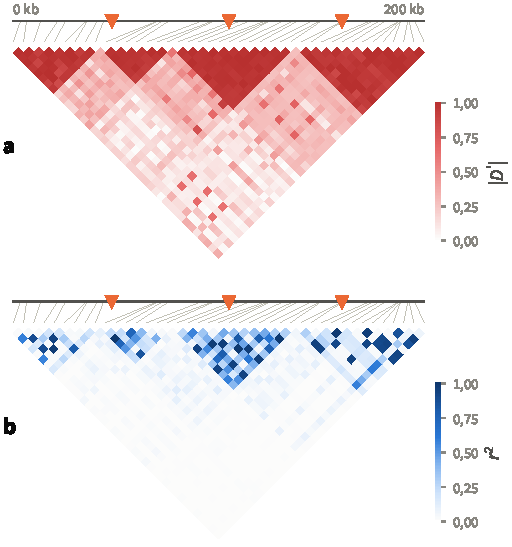
\includegraphics[width=0.78\linewidth]{figuras/cap10/ld_heatmap.pdf}
\caption[Mapa de calor del desequilibrio de ligamiento]{Mapa de LD al estilo de Haploview para 41 SNP en una región simulada de \SI{200}{kb} (600 haplotipos), con tres puntos calientes de recombinación (triángulos naranjas). Cada rombo representa un par de SNP: el del vértice superior de cada triángulo compara vecinos inmediatos, y hacia abajo se comparan SNP cada vez más alejados. Las líneas grises conectan cada SNP con su posición física. \textbf{a}: $|D'|$; dentro de cada bloque casi todos los pares tienen $|D'|\approx1$ (rojo oscuro), porque los haplotipos del bloque descienden de pocos ancestros sin recombinación entre ellos, y las fronteras coinciden con los puntos calientes. \textbf{b}: $r^2$ para los mismos pares; es mucho más irregular, porque dos SNP pueden estar en LD completo ($|D'|=1$) y aun así tener $r^2$ bajo si sus frecuencias alélicas son muy distintas. $D'$ revela la historia de recombinación; $r^2$, la capacidad de un SNP para sustituir a otro en un estudio de asociación. Simulación: mosaico de siete haplotipos fundadores por bloque (\archivo{figuras/cap10/generar.py}).}
\label{fig:10-ldmapa}
\end{figure}

Estas observaciones tuvieron una consecuencia práctica enorme: si los alelos de un bloque se heredan en unas pocas combinaciones, no hace falta genotipar todos los SNP; basta con unos pocos \emph{SNP etiqueta} (\ingles{tag SNPs}) que capturen, vía $r^2$, a los demás. El Proyecto Internacional HapMap se propuso catalogar ese patrón de LD en todo el genoma: su primera fase genotipó más de un millón de SNP en 269 individuos de cuatro poblaciones \parencite{c10-hapmap2005}, y sirvió para diseñar los chips de genotipado que harían posibles los primeros GWAS. Una década después, el Proyecto 1000 Genomas secuenció a 2504 personas de 26 poblaciones y construyó un panel de referencia de más de 88 millones de variantes \parencite{c10-1000g2015}. Con paneles así se practica la \emph{imputación}: a partir de los SNP genotipados con un chip y de los haplotipos de referencia, se predicen probabilísticamente los genotipos de millones de variantes no genotipadas, aprovechando precisamente el LD.

\begin{codigo}[ld.py]
import numpy as np

def ld(h1, h2):
    """D, D' y r^2 entre dos columnas de haplotipos 0/1."""
    pA, pB = h1.mean(), h2.mean()
    D = (h1 & h2).mean() - pA * pB
    if D >= 0:
        Dmax = min(pA * (1 - pB), (1 - pA) * pB)
    else:
        Dmax = min(pA * pB, (1 - pA) * (1 - pB))
    r2 = D ** 2 / (pA * (1 - pA) * pB * (1 - pB))
    return D, D / Dmax, r2

# H: matriz (haplotipos x SNP) de 0/1, p. ej., de un VCF faseado
# R2 = np.corrcoef(H.T) ** 2   # todos los r^2 de una vez
\end{codigo}

\begin{cuidado}[Genotipos no son haplotipos]
Un chip o una llamada de variantes estándar dan \emph{genotipos}, no haplotipos: sabemos que un individuo es $Aa$ y $Bb$, pero no si sus cromosomas son $AB/ab$ o $Ab/aB$. Estimar la fase (\ingles{phasing}) es un problema estadístico en sí mismo. Calcular $r^2$ a partir de dosis genotípicas (la correlación entre columnas $0/1/2$) es una aproximación útil y es lo que hacen herramientas como PLINK por defecto, pero $D'$ requiere haplotipos o una estimación de ellos.
\end{cuidado}

\subsection{Estructura poblacional y \texorpdfstring{$F_{ST}$}{FST}}

La \cref{sec:10-hw} supuso una población panmíctica. La humanidad no lo es: la geografía, la historia y la cultura hacen que las personas se apareen preferentemente con otras de su misma región, y las frecuencias alélicas derivan de manera independiente en cada grupo. \textcite{c10-wright1931} cuantificó esta subdivisión con el \emph{índice de fijación} $F_{ST}$: la reducción de heterocigosidad dentro de las subpoblaciones respecto a la que tendría la población total si fuera panmíctica,
\begin{equation}\label{eq:10-fst}
F_{ST} = \frac{H_T - H_S}{H_T} = \frac{\Var(p_k)}{\bar p\,(1-\bar p)}.
\end{equation}

\begin{simbolos}
\simbolo{$H_T$}{Heterocigosidad esperada con las frecuencias de la población total, $2\bar p(1-\bar p)$.}
\simbolo{$H_S$}{Promedio de las heterocigosidades esperadas dentro de cada subpoblación, $2p_k(1-p_k)$.}
\simbolo{$p_k,\ \bar p$}{Frecuencia alélica en la subpoblación $k$ y su media ponderada.}
\end{simbolos}

La segunda forma muestra que $F_{ST}$ es la varianza de las frecuencias entre subpoblaciones normalizada por su máximo posible. En la deriva de Wright-Fisher, subpoblaciones aisladas de tamaño $N$ acumulan $F_{ST}\approx 1-(1-1/2N)^t\approx t/2N$ al cabo de $t$ generaciones de separación: es el mismo $F_t$ de la \cref{eq:10-ibd}. Estimar $F_{ST}$ con muestras finitas requiere corregir el sesgo que introduce el propio muestreo; el estimador estándar es el de \textcite{c10-weir1984}, que descompone la varianza de las frecuencias en componentes entre poblaciones, entre individuos y dentro de individuos. Entre continentes, $F_{ST}$ humano es del orden de $0{,}1$; dentro de Europa, del orden de $0{,}01$ o menos.

\subsection{Análisis de componentes principales de genotipos}

Una medida resumen como $F_{ST}$ exige saber de antemano a qué población pertenece cada individuo. A menudo no lo sabemos, o las poblaciones no son discretas. El análisis de componentes principales (PCA) invierte el problema: encuentra, sin etiquetas, los ejes de mayor variación de la matriz de genotipos. \textcite{c10-patterson2006} le dieron un tratamiento estadístico riguroso.

\begin{definicion}{PCA de genotipos}{10-pca}
Sea $G$ la matriz $n\times M$ de genotipos ($g_{ij}\in\{0,1,2\}$) de $n$ individuos en $M$ SNP, y $\hat p_j$ la frecuencia alélica del SNP $j$. Se estandariza cada columna,
\begin{equation}\label{eq:10-zpca}
Z_{ij} = \frac{g_{ij}-2\hat p_j}{\sqrt{2\hat p_j(1-\hat p_j)}},
\qquad
\Psi = \frac{1}{M}\,ZZ^{\top} = \sum_{k} \lambda_k\, \mathbf{u}_k\mathbf{u}_k^{\top},
\end{equation}
y las coordenadas del individuo $i$ en el componente $k$ son $\sqrt{\lambda_k}\,u_{ik}$.
\end{definicion}

\begin{simbolos}
\simbolo{$Z$}{Matriz de genotipos centrada y escalada: cada SNP con media 0 y varianza 1 bajo HWE.}
\simbolo{$\Psi$}{Matriz $n\times n$ de parentesco genómico (GRM); $\Psi_{ii'}$ mide cuántos alelos comparten $i$ e $i'$ por encima de lo esperado al azar.}
\simbolo{$\lambda_k,\ \mathbf{u}_k$}{Autovalores y autovectores de $\Psi$, ordenados de mayor a menor.}
\end{simbolos}

La estandarización de la \cref{eq:10-zpca} da el mismo peso a cada SNP en términos de su varianza esperada, de modo que los SNP raros (cuya varianza es pequeña) no quedan ahogados por los comunes. La descomposición de $\Psi$ es, en la práctica, una descomposición en valores singulares de $Z$, lo que permite calcularla con miles de individuos y cientos de miles de SNP. Si no hubiera estructura, todos los autovalores serían parecidos; con $K$ poblaciones, aparecen $K-1$ autovalores destacados. \textcite{c10-patterson2006} mostraron cómo decidir cuántos son significativos comparándolos con la distribución de Tracy-Widom, y descubrieron un fenómeno de umbral: la estructura solo es detectable si $F_{ST}$ supera aproximadamente $1/\sqrt{nM}$. Con \num{1000} individuos y \num{100000} SNP, eso es $F_{ST}\approx10^{-4}$: el PCA puede separar poblaciones que ningún otro indicador distinguiría.

\begin{figure}[t]
\centering
\begin{tikzpicture}
\begin{groupplot}[group style={group size=2 by 1, horizontal sep=15mm},
   curso, height=5.0cm]
  \nextgroupplot[width=7.6cm, xlabel={PC1 (\SI{3,0}{\percent} de la varianza)}, ylabel={PC2 (\SI{1,4}{\percent})},
     xmin=-0.22, xmax=0.36, ymin=-0.24, ymax=0.36, legend pos=north east, legend columns=2,
     title={a. Individuos en los dos primeros ejes}, xtick={-0.2,0,0.2}, ytick={-0.2,0,0.2}]
  \addplot[only marks, mark=*, mark size=1.1pt, azul, fill opacity=0.6, draw opacity=0.6] table[x=pc1,y=pc2] {figuras/cap10/pca_A.dat}; \addlegendentry{población A}
  \addplot[only marks, mark=*, mark size=1.1pt, naranja, fill opacity=0.6, draw opacity=0.6] table[x=pc1,y=pc2] {figuras/cap10/pca_B.dat}; \addlegendentry{población B}
  \addplot[only marks, mark=*, mark size=1.1pt, aqua, fill opacity=0.6, draw opacity=0.6] table[x=pc1,y=pc2] {figuras/cap10/pca_C.dat}; \addlegendentry{población C}
  \addplot[only marks, mark=diamond*, mark size=1.6pt, violeta] table[x=pc1,y=pc2] {figuras/cap10/pca_M.dat}; \addlegendentry{mezcla A$\times$B}
  \nextgroupplot[width=5.0cm, ybar, bar width=5pt, xlabel={componente $k$}, ylabel={autovalor $\lambda_k$},
     ymin=0, ymax=15, xtick={1,2,3,4,5,6,7,8,9,10}, xticklabels={1,2,3,,5,,,,,10}, grid=none,
     title={b. Autovalores}]
  \addplot[fill=azul, draw=azulprofundo] table[x=k,y=ev] {figuras/cap10/pca_ev.dat};
\end{groupplot}
\end{tikzpicture}
\caption[PCA de tres poblaciones]{PCA de 450 individuos simulados en unos \num{6000} SNP. Tres poblaciones (130 individuos cada una) derivaron desde un ancestro común con el modelo de Balding-Nichols; C está más diferenciada ($F_{ST}$ de Weir-Cockerham: A--B $0{,}020$, A--C $0{,}040$, B--C $0{,}040$). Otros 60 individuos tienen ancestría mixta A$\times$B en proporciones aleatorias. \textbf{a}: PC1 separa a C de las demás y PC2 separa a A de B; los individuos mezclados forman un puente entre A y B, y su posición en PC2 correlaciona en $0{,}98$ con su fracción real de ancestría A. \textbf{b}: con tres poblaciones aparecen exactamente dos autovalores destacados; los demás forman el ``mar'' de ruido ($\lambda\approx1{,}5$) que describe la teoría de matrices aleatorias.}
\label{fig:10-pca}
\end{figure}

El resultado más célebre de esta técnica es el de \textcite{c10-novembre2008}, que aplicaron PCA a genotipos de más de mil europeos y encontraron que, al rotar ligeramente los dos primeros componentes, la nube de individuos reproducía el mapa de Europa: los genes reflejan la geografía. La interpretación es la del modelo de aislamiento por distancia: cuando las personas se aparean con sus vecinos, las frecuencias alélicas varían suavemente en el espacio y los primeros componentes principales recuperan las coordenadas geográficas.

\begin{codigo}[pca\_genotipos.py]
import numpy as np

def pca_genotipos(G, k=10):
    """G: n x M con 0/1/2. Devuelve coordenadas y autovalores."""
    p = G.mean(axis=0) / 2
    ok = (p > 0.01) & (p < 0.99)          # descartar monomórficos
    Z = (G[:, ok] - 2 * p[ok]) / np.sqrt(2 * p[ok] * (1 - p[ok]))
    U, S, _ = np.linalg.svd(Z, full_matrices=False)
    lam = S ** 2 / Z.shape[1]                    # autovalores de Psi
    return U[:, :k] * np.sqrt(lam[:k]), lam
\end{codigo}

\begin{cuidado}[El PCA también ve el LD]
El PCA supone implícitamente que los SNP son independientes. Una región larga de LD fuerte (como el complejo HLA en el cromosoma 6, o una inversión cromosómica polimórfica) aporta cientos de SNP casi idénticos y puede ``secuestrar'' un componente entero, que entonces refleja el genotipo de esa región y no la ancestría. Por eso, antes del PCA, se \emph{poda} el conjunto de SNP para eliminar pares con $r^2$ alto (en PLINK, \texttt{--indep-pairwise}) y se excluyen las regiones de LD extenso conocidas.
\end{cuidado}

% ---------------------------------------------------------------------
\section{GWAS: Manhattan, QQ plots y corrección múltiple}\label{sec:10-gwas}
% ---------------------------------------------------------------------
\enlacecolab{modulo-10-poblaciones-gwas/10.3_gwas.ipynb}{10.3 · GWAS}

\begin{intuicion}[La encuesta de los paraguas]
Suponga que quiere saber si llevar paraguas protege contra los resfriados. Encuesta a mil personas en dos ciudades: una lluviosa, donde casi todos llevan paraguas, y otra seca. Si en la ciudad lluviosa, por su clima frío, también hay más resfriados, encontrará una asociación fuerte entre paraguas y resfriados, sin que el paraguas tenga nada que ver: la ciudad es una variable de confusión que se correlaciona con ambos. Un estudio de asociación genética es exactamente esta encuesta repetida un millón de veces, una por cada variante, y con el mismo peligro: si los casos y los controles provienen en proporciones distintas de poblaciones con frecuencias alélicas distintas, \emph{todas} las variantes diferenciadas entre esas poblaciones parecerán asociadas con la enfermedad. La mitad de esta sección trata de cómo encontrar asociaciones; la otra mitad, de cómo no engañarse.
\end{intuicion}

\subsection{La idea y el diseño}

Un estudio de asociación del genoma completo (GWAS, \ingles{genome-wide association study}) prueba, una a una, cientos de miles o millones de variantes para detectar las que difieren en frecuencia entre casos y controles, o que se correlacionan con un rasgo cuantitativo. No necesita familias ni una hipótesis previa sobre qué genes intervienen: se apoya en que, gracias al LD, una variante genotipada ``etiqueta'' a sus vecinas no genotipadas, incluida la causal. La premisa biológica es la hipótesis de \emph{enfermedad común, variante común}: buena parte del riesgo genético de las enfermedades frecuentes se debería a variantes frecuentes, cada una con un efecto pequeño.

\begin{historia}[El estudio que abrió la era de los GWAS]
En 2007, el Wellcome Trust Case Control Consortium publicó un estudio con unos \num{2000} casos de cada una de siete enfermedades comunes (trastorno bipolar, enfermedad coronaria, enfermedad de Crohn, hipertensión, artritis reumatoide y diabetes de tipos 1 y 2) y \num{3000} controles compartidos, genotipados en unos \num{500000} SNP \parencite{c10-wtccc2007}. Encontró 24 señales de asociación independientes con $p<5\times10^{-7}$, muchas en genes nunca antes relacionados con esas enfermedades. Tan importante como los hallazgos fue el método: el artículo estableció buena parte del control de calidad, el análisis de estratificación y el uso de gráficos QQ que se volvieron estándar. Diez años después, los GWAS habían identificado miles de loci asociados con cientos de rasgos \parencite{c10-visscher2017}.
\end{historia}

La \cref{fig:10-flujo} resume las etapas de un GWAS típico. Todas son importantes, pero dos concentran la mayor parte de los errores: el control de la estructura poblacional y la corrección por comparaciones múltiples.

\begin{figure}[t]
\centering
\begin{tikzpicture}[font=\sffamily\small, node distance=4mm and 5mm,
   paso/.style={caja=#1, minimum width=2.5cm, minimum height=1.25cm, text width=2.3cm}]
  \node[paso=azul] (g) {Genotipado\\{\scriptsize chip o secuencia}};
  \node[paso=azul, right=of g] (qc) {Control de calidad\\{\scriptsize tasa de llamada, MAF, HWE}};
  \node[paso=azul, right=of qc] (imp) {Faseado e imputación\\{\scriptsize panel de referencia}};
  \node[paso=aqua, right=of imp] (pc) {Estructura\\{\scriptsize PCA, GRM, parentesco}};
  \node[paso=naranja, below=9mm of pc] (as) {Asociación\\{\scriptsize regresión por variante}};
  \node[paso=naranja, left=of as] (mt) {Corrección múltiple\\{\scriptsize $5\times10^{-8}$, FDR}};
  \node[paso=naranja, left=of mt] (vis) {Diagnóstico\\{\scriptsize QQ, $\lambda_{GC}$, Manhattan}};
  \node[paso=violeta, left=of vis] (rep) {Replicación y mapeo fino};
  \draw[flecha] (g) -- (qc); \draw[flecha] (qc) -- (imp); \draw[flecha] (imp) -- (pc);
  \draw[flecha] (pc) -- (as); \draw[flecha] (as) -- (mt); \draw[flecha] (mt) -- (vis); \draw[flecha] (vis) -- (rep);
\end{tikzpicture}
\caption[Flujo de trabajo de un GWAS]{Etapas de un GWAS. En azul, la preparación de los datos: el control de calidad elimina individuos y variantes con muchos datos faltantes, frecuencias muy bajas o desviaciones extremas de Hardy-Weinberg (\cref{sec:10-hw}); la imputación aprovecha el LD con un panel de referencia (\cref{sec:10-ld}) para pasar de cientos de miles a decenas de millones de variantes. En verde, la estructura poblacional, que entra en el modelo como covariables. En naranja, el análisis estadístico propiamente dicho. En violeta, lo que ocurre después: toda asociación debe replicarse en una muestra independiente, y la variante más significativa rara vez es la causal.}
\label{fig:10-flujo}
\end{figure}

\subsection{El modelo aditivo}

Para cada variante $j$ se ajusta un modelo de regresión en el que el genotipo entra como el número de copias del alelo de efecto, $g_{ij}\in\{0,1,2\}$ (o su dosis imputada, un número real entre 0 y 2). Para un rasgo cuantitativo,
\begin{equation}\label{eq:10-lineal}
y_i = \alpha + \beta_j\, g_{ij} + \boldsymbol\gamma^{\top}\mathbf{c}_i + \varepsilon_i,\qquad \varepsilon_i\sim\mathcal N(0,\sigma^2),
\end{equation}
y para una enfermedad (caso/control), la regresión logística
\begin{equation}\label{eq:10-logistica}
\log\frac{\Prob(y_i=1)}{1-\Prob(y_i=1)} = \alpha + \beta_j\, g_{ij} + \boldsymbol\gamma^{\top}\mathbf{c}_i ,\qquad \mathrm{OR}_j=e^{\beta_j}.
\end{equation}
La hipótesis nula es $\beta_j=0$, y se contrasta con el estadístico de Wald $z_j=\hat\beta_j/\widehat{\mathrm{se}}(\hat\beta_j)$, que bajo la nula es aproximadamente normal estándar (o, equivalentemente, $z_j^2\sim\chi^2_1$).

\begin{simbolos}
\simbolo{$y_i$}{Fenotipo del individuo $i$: un valor continuo o un indicador de enfermedad (1 = caso).}
\simbolo{$g_{ij}$}{Número de copias del alelo de efecto en la variante $j$.}
\simbolo{$\beta_j$}{Efecto aditivo: cambio en el rasgo (o en el logaritmo de las probabilidades) por cada copia adicional.}
\simbolo{$\mathbf{c}_i,\ \boldsymbol\gamma$}{Covariables (sexo, edad, componentes principales) y sus coeficientes.}
\simbolo{$\mathrm{OR}_j$}{Razón de probabilidades (\ingles{odds ratio}) por copia del alelo.}
\end{simbolos}

¿Por qué aditivo? Porque es el modelo con un solo grado de libertad que mejor potencia tiene frente a una amplia gama de modelos verdaderos: una variante dominante o recesiva sigue produciendo una tendencia monótona en la media de los tres genotipos, que la regresión lineal detecta. Además, la varianza del rasgo explicada por una variante aditiva tiene una forma sencilla:
\begin{equation}\label{eq:10-q2}
q^2_j = \frac{2p_j(1-p_j)\,\beta_j^2}{\sigma_y^2}, \qquad \E[z_j^2]\approx 1 + \frac{n\,q_j^2}{1-q_j^2}.
\end{equation}

\begin{simbolos}
\simbolo{$q_j^2$}{Fracción de la varianza fenotípica explicada por la variante $j$.}
\simbolo{$2p_j(1-p_j)$}{Varianza del genotipo bajo HWE; las variantes raras explican poca varianza aunque su efecto sea grande.}
\simbolo{$n q^2/(1-q^2)$}{Parámetro de no centralidad del $\chi^2_1$: determina la potencia.}
\end{simbolos}

La \cref{eq:10-q2} explica por qué los GWAS modernos necesitan cientos de miles de participantes. Una variante con $p=0{,}3$ que desplaza el rasgo $0{,}05$ desviaciones estándar por copia explica $q^2=2\cdot0{,}3\cdot0{,}7\cdot0{,}05^2=0{,}00105$, apenas una milésima de la varianza. Con un umbral $\alpha=5\times10^{-8}$ ($\chi^2_1>29{,}7$), para detectarla con \SI{80}{\percent} de potencia hacen falta unos \num{40000} individuos; si explicara la mitad de eso, unos \num{79000} (\cref{fig:10-bh}b).

\subsection{Estratificación poblacional}

Volvamos a los paraguas. Suponga que la muestra mezcla dos poblaciones con frecuencias alélicas distintas en muchas variantes, y que el rasgo también difiere en promedio entre ellas, por razones genéticas o ambientales. Entonces toda variante diferenciada entre las poblaciones mostrará una asociación con el rasgo, aunque no tenga ningún efecto. Este sesgo, la \emph{estratificación poblacional}, no afecta a unas pocas variantes sino a todo el genoma, y deja una huella característica: infla la distribución completa de los estadísticos de prueba.

\paragraph{Control genómico} \textcite{c10-devlin1999} propusieron medir esa inflación con la mediana. Bajo la nula, $z^2\sim\chi^2_1$, cuya mediana es $0{,}4549$. Si la estratificación multiplica todos los estadísticos por un factor aproximadamente constante,
\begin{equation}\label{eq:10-lambda}
\hat\lambda_{GC} = \frac{\operatorname{mediana}(z_1^2,\dots,z_M^2)}{0{,}4549},\qquad \tilde z_j^2 = \frac{z_j^2}{\hat\lambda_{GC}},
\end{equation}
y dividir por $\hat\lambda_{GC}$ restaura la calibración. La mediana es robusta: las pocas variantes verdaderamente asociadas apenas la mueven. Un $\lambda_{GC}$ cercano a 1 indica un estudio bien controlado. Hay una salvedad importante: en rasgos muy poligénicos con muestras enormes, miles de variantes causales de efecto diminuto inflan legítimamente la mediana, y un $\lambda_{GC}$ de $1{,}1$ o más no implica necesariamente confusión.

\paragraph{Componentes principales} La corrección por $\lambda_{GC}$ es uniforme, pero la estratificación no lo es: afecta más a las variantes más diferenciadas entre poblaciones. \textcite{c10-price2006} propusieron EIGENSTRAT: calcular los ejes principales de variación genética (\cref{eq:10-zpca}) y eliminar de genotipos y fenotipos la parte explicada por ellos, lo que equivale a incluir los primeros componentes como covariables $\mathbf{c}_i$ en la \cref{eq:10-lineal}. Así, cada variante se corrige en proporción a su propia diferenciación.

\begin{ejemplo}{Una asociación espuria y su corrección}{10-estrat}
Simulamos \num{2000} individuos de dos poblaciones (\num{1000} de cada una, $F_{ST}\approx0{,}02$) y \num{10000} SNP, con 10 variantes causales de efecto pequeño y un rasgo que, además, es $0{,}3$ desviaciones estándar más alto en la segunda población. La regresión ingenua da $\hat\lambda_{GC}=1{,}86$: 148 variantes superan $p<10^{-3}$, cuando por azar se esperarían 10 más unas pocas causales. El primer componente principal correlaciona en $0{,}997$ con la población de origen; al incluir dos componentes como covariables, $\hat\lambda_{GC}=0{,}98$ y quedan 18 variantes con $p<10^{-3}$ (\cref{fig:10-qq}b). En esta simulación modesta, las variantes que superan $5\times10^{-8}$ son causales en ambos análisis: la inflación se concentra en la zona intermedia de valores $p$. Pero la inflación crece con el tamaño de muestra (la no centralidad espuria es proporcional a $n$), y en un estudio diez veces mayor esas mismas diferencias de frecuencia producirían rascacielos falsos en el gráfico Manhattan.
\end{ejemplo}

\paragraph{Modelos lineales mixtos} Los componentes principales capturan bien la estructura a gran escala, pero no el parentesco críptico (primos lejanos en la muestra) ni la estructura fina. Los modelos mixtos modelan toda la similitud genética a la vez:
\begin{equation}\label{eq:10-lmm}
\mathbf{y} = X\boldsymbol\gamma + \mathbf{g}_j\beta_j + \mathbf{u} + \boldsymbol\varepsilon,\qquad
\mathbf{u}\sim\mathcal N\!\left(\mathbf 0,\ \sigma_g^2\,\Psi\right),\quad
\boldsymbol\varepsilon\sim\mathcal N\!\left(\mathbf 0,\ \sigma_e^2 I\right).
\end{equation}

\begin{simbolos}
\simbolo{$\mathbf{u}$}{Efecto genético poligénico aleatorio: la suma de los efectos de todas las demás variantes.}
\simbolo{$\Psi$}{Matriz de parentesco genómico de la \cref{eq:10-zpca}: individuos más emparentados tienen efectos $\mathbf u$ más correlacionados.}
\simbolo{$\sigma_g^2,\ \sigma_e^2$}{Varianzas genética y residual; $\sigma_g^2/(\sigma_g^2+\sigma_e^2)$ es la heredabilidad atribuible a los SNP.}
\end{simbolos}

\textcite{c10-yang2011} popularizaron, con el programa GCTA, el uso de la matriz $\Psi$ calculada con SNP y la estimación por máxima verosimilitud restringida (REML) de la varianza que todos los SNP explican conjuntamente, la llamada heredabilidad SNP. Ajustar la \cref{eq:10-lmm} para cada una de millones de variantes era prohibitivo con los algoritmos clásicos, cuyo coste crece con el cubo del número de individuos; \textcite{c10-loh2015} desarrollaron BOLT-LMM, que evita construir y factorizar $\Psi$ mediante métodos iterativos y un modelo bayesiano de efectos, y mostraron que aumenta la potencia de asociación en cohortes grandes.

\begin{figure}[t]
\centering
\begin{tikzpicture}
\begin{groupplot}[group style={group size=2 by 1, horizontal sep=15mm},
   curso, width=6.3cm, height=5.2cm, xlabel={$-\log_{10} p$ esperado}]
  \nextgroupplot[xmin=0, xmax=5.4, ymin=0, ymax=34, ylabel={$-\log_{10} p$ observado},
     title={a. GWAS de la \cref{fig:10-manhattan}}, legend pos=north west]
  \addplot[name path=hi, draw=none, forget plot] table[x=e,y=hi] {figuras/cap10/qq_banda90k.dat};
  \addplot[name path=lo, draw=none, forget plot] table[x=e,y=lo] {figuras/cap10/qq_banda90k.dat};
  \addplot[papel!80!gris, forget plot] fill between[of=hi and lo];
  \addplot[gris, dashed, domain=0:5.4, forget plot] {x};
  \addplot[only marks, mark=*, mark size=0.9pt, azul] table[x=e,y=o] {figuras/cap10/qq_manhattan.dat};
  \addlegendentry{$\lambda_{GC}=1{,}01$}
  \nextgroupplot[xmin=0, xmax=4.4, ymin=0, ymax=27, ylabel={},
     title={b. Estratificación}, legend pos=north west]
  \addplot[name path=hi, draw=none, forget plot] table[x=e,y=hi] {figuras/cap10/qq_banda10k.dat};
  \addplot[name path=lo, draw=none, forget plot] table[x=e,y=lo] {figuras/cap10/qq_banda10k.dat};
  \addplot[papel!80!gris, forget plot] fill between[of=hi and lo];
  \addplot[gris, dashed, domain=0:4.4, forget plot] {x};
  \addplot[only marks, mark=*, mark size=0.9pt, rojo] table[x=e,y=o] {figuras/cap10/qq_naive.dat};
  \addlegendentry{sin corregir, $\lambda_{GC}=1{,}86$}
  \addplot[only marks, mark=*, mark size=0.9pt, aqua] table[x=e,y=o] {figuras/cap10/qq_pc.dat};
  \addlegendentry{2 PCs, $\lambda_{GC}=0{,}98$}
\end{groupplot}
\end{tikzpicture}
\caption[Gráficos QQ]{Gráficos cuantil-cuantil de los valores $p$: cada punto compara el $k$-ésimo valor $p$ más pequeño observado con el esperado bajo la hipótesis nula global, $(k-0{,}5)/M$. La banda gris es el intervalo del \SI{95}{\percent} de cada estadístico de orden bajo la nula, y la diagonal es la identidad. \textbf{a}: estudio bien calibrado con señales reales; los puntos siguen la diagonal casi hasta el final y solo se despegan en la cola, donde están las verdaderas asociaciones. \textbf{b}: estudio con estratificación (\cref{ej:10-estrat}); sin corrección (rojo), los puntos se separan de la diagonal desde el principio, síntoma de inflación de \emph{todo} el genoma; con dos componentes principales como covariables (verde), la nube vuelve a la banda. Se muestran todos los puntos de la cola y una submuestra del resto.}
\label{fig:10-qq}
\end{figure}

\subsection{Comparaciones múltiples}

Con un millón de pruebas independientes y el umbral clásico $\alpha=0{,}05$, esperaríamos \num{50000} falsos positivos. Hay dos filosofías para evitarlo.

\paragraph{Error por familia: Bonferroni y $5\times10^{-8}$} La tasa de error por familia (FWER) es la probabilidad de cometer \emph{al menos un} falso positivo. Por la desigualdad de Boole, si cada una de $M$ pruebas se realiza al nivel $\alpha/M$,
\begin{equation}\label{eq:10-bonferroni}
\mathrm{FWER} = \Prob\Big(\bigcup_{j=1}^{M}\{p_j\le \alpha/M\}\Big) \le \sum_{j=1}^{M}\frac{\alpha}{M} = \alpha ,
\end{equation}
sin ningún supuesto sobre la dependencia entre pruebas. En un GWAS las pruebas no son independientes: el LD hace que muchas variantes vecinas sean casi redundantes, y Bonferroni sobre el número bruto de variantes sería demasiado conservador. \textcite{c10-peer2008} estimaron el número \emph{efectivo} de pruebas independientes al evaluar prácticamente todas las variantes comunes del genoma en poblaciones de ascendencia europea, que resultó del orden de un millón. De ahí el umbral convencional de significación genómica, $0{,}05/10^6=5\times10^{-8}$. En poblaciones africanas, con LD más corto, el número efectivo de pruebas es mayor y el umbral debería ser algo más estricto; y con variantes raras de secuenciación completa, también.

\paragraph{Tasa de falsos descubrimientos} En estudios exploratorios, controlar la probabilidad de un solo error puede ser excesivo. \textcite{c10-benjamini1995} propusieron controlar la \emph{tasa de falsos descubrimientos} (FDR): la proporción esperada de falsos positivos entre las pruebas declaradas significativas.

\begin{teorema}{Procedimiento de Benjamini-Hochberg}{10-bh}
Se ordenan los valores $p$ de menor a mayor, $p_{(1)}\le\dots\le p_{(M)}$, y se busca
\begin{equation}\label{eq:10-bh}
k^\ast = \max\left\{k:\ p_{(k)} \le \frac{k}{M}\,\alpha\right\}.
\end{equation}
Se rechazan las hipótesis correspondientes a $p_{(1)},\dots,p_{(k^\ast)}$. Si las pruebas son independientes, el procedimiento garantiza $\mathrm{FDR}\le \frac{M_0}{M}\alpha\le\alpha$, donde $M_0$ es el número de hipótesis nulas verdaderas.
\end{teorema}

\begin{simbolos}
\simbolo{$p_{(k)}$}{$k$-ésimo valor $p$ más pequeño.}
\simbolo{$k^\ast$}{Número de descubrimientos: el mayor rango cuyo valor $p$ cae bajo la recta $k\alpha/M$.}
\simbolo{$M_0$}{Número (desconocido) de hipótesis nulas ciertas.}
\end{simbolos}

\begin{ejemplo}{Bonferroni frente a Benjamini-Hochberg}{10-bh}
Diez pruebas dan, ordenados, los valores $p$: $0{,}0001$, $0{,}0008$, $0{,}0021$, $0{,}0042$, $0{,}0110$, $0{,}0290$, $0{,}0480$, $0{,}0730$, $0{,}21$ y $0{,}62$. Con $\alpha=0{,}05$, Bonferroni exige $p\le0{,}005$ y rechaza 4. Los umbrales de Benjamini-Hochberg son $0{,}005$, $0{,}010$, $0{,}015$, \dots, $0{,}050$; el sexto valor ($0{,}0290\le0{,}030$) todavía cae bajo su umbral y el séptimo ($0{,}048>0{,}035$) ya no, de modo que $k^\ast=6$ y se rechazan seis hipótesis. Observe que no es necesario que todos los valores anteriores cumplan su propio umbral: lo que cuenta es el \emph{mayor} $k$ que lo hace.
\end{ejemplo}

\begin{figure}[t]
\centering
\begin{tikzpicture}
\begin{groupplot}[group style={group size=2 by 1, horizontal sep=15mm},
   curso, width=6.4cm, height=5.0cm]
  \nextgroupplot[ymode=log, xmin=0, xmax=40, ymin=1e-8, ymax=1, xlabel={rango $k$},
     ylabel={valor $p_{(k)}$}, title={a. Umbrales ($M=200$, $\alpha=0{,}05$)},
     legend style={at={(0.98,0.03)},anchor=south east}, unbounded coords=discard,
     ytick={1e-8,1e-6,1e-4,1e-2,1}]
  \addplot[only marks, mark=*, mark size=1.4pt, azul,
     x filter/.expression={\thisrow{real}>0.5 ? x : nan}] table[x=k,y=p] {figuras/cap10/bh.dat};
  \addlegendentry{efecto real}
  \addplot[only marks, mark=o, mark size=1.5pt, gris,
     x filter/.expression={\thisrow{real}<0.5 ? x : nan}] table[x=k,y=p] {figuras/cap10/bh.dat};
  \addlegendentry{nula verdadera}
  \addplot[naranja, thick, domain=1:40, samples=40] {0.05*x/200};
  \addlegendentry{BH: $k\alpha/M$}
  \addplot[rojo, thick, dashed, domain=0:40] {0.05/200};
  \addlegendentry{Bonferroni: $\alpha/M$}
  \nextgroupplot[xmode=log, xmin=1e3, xmax=1e6, ymin=0, ymax=1.02, xlabel={tamaño de muestra $n$},
     ylabel={potencia a $5\times10^{-8}$}, title={b. Potencia}, legend pos=north west,
     legend style={font=\sffamily\tiny}]
  \addplot[azulnoche] table[x=n,y=q005] {figuras/cap10/potencia.dat}; \addlegendentry{$q^2=0{,}5\,\%$}
  \addplot[azul] table[x=n,y=q002] {figuras/cap10/potencia.dat}; \addlegendentry{$q^2=0{,}2\,\%$}
  \addplot[violeta] table[x=n,y=q001] {figuras/cap10/potencia.dat}; \addlegendentry{$q^2=0{,}1\,\%$}
  \addplot[naranja] table[x=n,y=q0005] {figuras/cap10/potencia.dat}; \addlegendentry{$q^2=0{,}05\,\%$}
  \draw[gris, dashed] (axis cs:1e3,0.8) -- (axis cs:1e6,0.8);
\end{groupplot}
\end{tikzpicture}
\caption[Corrección múltiple y potencia]{\textbf{a}: los 40 valores $p$ más pequeños de 200 pruebas simuladas, de las cuales 20 tienen un efecto real (azul). Bonferroni (línea roja discontinua) declara 5 descubrimientos; Benjamini-Hochberg (recta naranja, que crece con el rango) declara 8, sin ningún falso positivo en este caso; y el umbral sin corregir $p<0{,}05$ declararía 25, de los cuales 7 serían falsos. \textbf{b}: potencia de una prueba $\chi^2_1$ al umbral genómico en función del tamaño de muestra, para variantes que explican distintas fracciones $q^2$ de la varianza (\cref{eq:10-q2}). La transición de potencia casi nula a casi total ocurre en menos de un orden de magnitud de $n$: con $q^2=0{,}1\,\%$, la potencia es del \SI{1}{\percent} con \num{10000} individuos y del \SI{95}{\percent} con \num{50000}.}
\label{fig:10-bh}
\end{figure}

\begin{codigo}[asociacion.py]
import numpy as np
from scipy import stats

def gwas_lineal(y, G, C=None):
    """Regresión marginal por SNP; C = covariables (n x k)."""
    n = len(y)
    Q = np.ones((n, 1))
    if C is not None:
        Q = np.column_stack([Q, C])
    Q, _ = np.linalg.qr(Q)
    yr = y - Q @ (Q.T @ y)                       # residualizar (FWL)
    Gr = G - Q @ (Q.T @ G)
    sxx = (Gr ** 2).sum(axis=0)
    b = Gr.T @ yr / sxx
    df = n - Q.shape[1] - 1
    se = np.sqrt(((yr ** 2).sum() - b ** 2 * sxx) / df / sxx)
    return b, 2 * stats.t.sf(np.abs(b / se), df)

def lambda_gc(p):
    return np.median(stats.chi2.isf(p, 1)) / stats.chi2.ppf(0.5, 1)

def benjamini_hochberg(p, alpha=0.05):
    o = np.argsort(p); M = len(p)
    ok = p[o] <= alpha * np.arange(1, M + 1) / M
    k = ok.nonzero()[0].max() + 1 if ok.any() else 0
    rechazo = np.zeros(M, bool); rechazo[o[:k]] = True
    return rechazo
\end{codigo}

La función \py{gwas_lineal} usa el teorema de Frisch-Waugh-Lovell: el coeficiente de un SNP en una regresión con covariables es igual al de la regresión simple entre los residuos del SNP y del fenotipo después de proyectar ambos fuera del espacio de las covariables. Así se prueban todas las variantes con dos productos de matrices, sin un bucle.

\subsection{Leer un gráfico Manhattan}

El resultado de un GWAS se resume en dos gráficos. El \emph{gráfico Manhattan} (\cref{fig:10-manhattan}) sitúa cada variante según su posición en el genoma y su $-\log_{10}p$: las asociaciones aparecen como rascacielos sobre un horizonte de ruido. El \emph{gráfico QQ} (\cref{fig:10-qq}) compara la distribución completa de los valores $p$ con la esperada bajo la nula y sirve de diagnóstico: una desviación temprana indica inflación; una desviación solo en la cola, señales reales.

\begin{figure}[t]
\centering
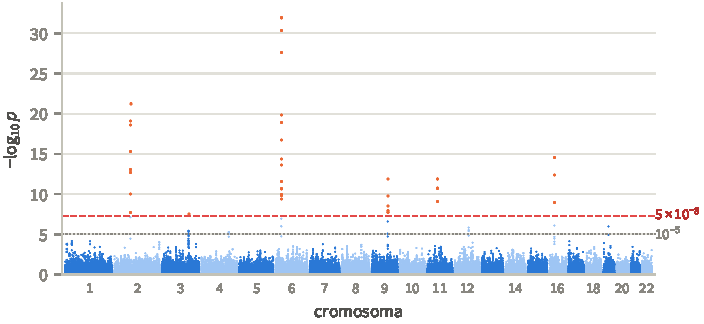
\includegraphics[width=\linewidth]{figuras/cap10/manhattan.pdf}
\caption[Gráfico Manhattan]{Gráfico Manhattan de un GWAS simulado con \num{89999} variantes en los 22 autosomas, cada una representada por su $-\log_{10}p$. La línea roja marca la significación genómica ($5\times10^{-8}$) y la punteada, el umbral ``sugestivo'' de $10^{-5}$. Treinta y cinco variantes (naranja) superan el umbral genómico, agrupadas en seis loci de los cromosomas 2, 3, 6, 9, 11 y 16; el pico más alto ($p=1{,}4\times10^{-32}$, cromosoma 6) imita la señal típica del complejo HLA en enfermedades autoinmunes. Cada pico es una torre y no una aguja aislada porque las variantes vecinas en LD con la causal heredan una parte de su señal, proporcional a su correlación. Las señales simuladas en los cromosomas 12 y 19 quedan en la zona sugestiva ($p\approx10^{-6}$): con este tamaño de muestra, el estudio no tiene potencia para declararlas. El factor de inflación es $\lambda_{GC}=1{,}01$.}
\label{fig:10-manhattan}
\end{figure}

Al leer un Manhattan conviene tener presentes tres advertencias. Primera: la variante con el valor $p$ más bajo de una torre (la variante ``líder'') no es necesariamente la causal; es solo la que mejor etiqueta a la causal en esta muestra, y la identificación de la variante causal requiere \emph{mapeo fino} estadístico y funcional. Segunda: el locus se nombra a menudo por el gen más cercano, pero la variante causal puede actuar sobre un gen a cientos de kilobases, a través de un elemento regulador. Tercera: un pico formado por una única variante aislada, sin vecinas que la acompañen, es sospechoso de ser un artefacto de genotipado.

\begin{consola}[GWAS con PLINK 2]
# 1. Control de calidad de variantes e individuos
plink2 --bfile crudo --geno 0.02 --mind 0.02 --maf 0.01 \
       --hwe 1e-6 --make-bed --out qc
# 2. Podar por LD y calcular 10 componentes principales
plink2 --bfile qc --indep-pairwise 200 50 0.2 --out podado
plink2 --bfile qc --extract podado.prune.in --pca 10 --out pcs
# 3. Asociación con las PCs como covariables
plink2 --bfile qc --pheno fenotipo.txt --covar pcs.eigenvec \
       --glm hide-covar --out gwas
\end{consola}

PLINK \parencite{c10-purcell2007} se convirtió en la navaja suiza del análisis de asociación: control de calidad, estadísticas de LD, PCA, pruebas de asociación y manejo de formatos, todo sobre un formato binario compacto (\archivo{.bed}/\archivo{.bim}/\archivo{.fam}). Su segunda generación \parencite{c10-chang2015} reescribió el núcleo con operaciones a nivel de bits y paralelismo, y lo aceleró en uno a varios órdenes de magnitud, lo que le permite trabajar con biobancos de cientos de miles de personas.

\subsection{Lo que los GWAS encontraron, y lo que falta}

Los resultados publicados se reúnen en el GWAS Catalog, mantenido por el NHGRI y el EBI, que recopila cientos de miles de asociaciones curadas a partir de miles de publicaciones y ofrece además un repositorio para depositar estadísticas resumidas completas \parencite{c10-sollis2023}. Esa masa de resultados ha confirmado que la mayoría de los rasgos complejos son \emph{altamente poligénicos}: miles de variantes, cada una con un efecto diminuto, casi siempre en regiones no codificantes \parencite{c10-visscher2017}.

\textcite{c10-manolio2009} plantearon el problema de la \emph{heredabilidad faltante}: para la estatura, cuya heredabilidad estimada en estudios de familias ronda el \SI{80}{\percent}, las decenas de loci conocidos entonces explicaban apenas un \SI{5}{\percent} de la varianza. Las explicaciones propuestas incluían variantes comunes de efecto demasiado pequeño para superar el umbral, variantes raras mal etiquetadas por los chips, variantes estructurales, interacciones y sobreestimaciones de la heredabilidad familiar. La primera explicación resultó ser la más importante: la heredabilidad SNP estimada con modelos como el de la \cref{eq:10-lmm} recupera una parte sustancial de la heredabilidad faltante, y cada aumento del tamaño de muestra ha traído nuevos loci, como predice la curva de potencia de la \cref{fig:10-bh}b.

\begin{cuidado}[Asociación no es causalidad (ni predicción universal)]
Un GWAS encuentra correlaciones entre variantes y rasgos en una población concreta. La mayoría de los estudios se ha hecho en personas de ascendencia europea, y como el LD y las frecuencias alélicas difieren entre poblaciones (\cref{sec:10-ld}), una variante etiqueta que funciona bien en una población puede no hacerlo en otra. Las puntuaciones de riesgo poligénico construidas con esos resultados pierden buena parte de su capacidad predictiva cuando se aplican a otras ascendencias. Diversificar las cohortes es hoy una prioridad científica, no solo ética.
\end{cuidado}

\begin{ideaclave}
Un GWAS es un millón de regresiones con un solo enemigo sistemático, la estructura poblacional, y un solo enemigo aleatorio, la multiplicidad. El gráfico QQ vigila al primero; el umbral de $5\times10^{-8}$, al segundo.
\end{ideaclave}

\begin{resumen}
\begin{itemize}
  \item Bajo apareamiento aleatorio, las frecuencias genotípicas son $p^2:2pq:q^2$ tras una sola generación (Hardy-Weinberg). Las desviaciones se contrastan con $\chi^2$ o, para variantes raras, con la prueba exacta; el coeficiente $F$ mide el déficit de heterocigotos.
  \item El modelo de Wright-Fisher es una cadena de Márkov binomial: la frecuencia es una martingala, un alelo neutral se fija con probabilidad igual a su frecuencia, y la heterocigosidad decae como $(1-1/2N_e)^t$. El tamaño efectivo es una media armónica dominada por los cuellos de botella.
  \item La difusión de Kimura da distribuciones, tiempos de fijación ($4N\ln2$ para $p=1/2$) y la probabilidad de fijación con selección; lo que importa es $4N_es$. El coalescente describe la misma deriva hacia atrás en el tiempo.
  \item El LD se mide con $D$, $D'$ (historia de recombinación) y $r^2$ (poder de sustitución entre marcadores); decae como $(1-c)^t$ y, en equilibrio con la deriva, $\E[r^2]\approx1/(1+4N_ec)$. Los puntos calientes de recombinación organizan el genoma en bloques de haplotipos.
  \item El PCA de la matriz de genotipos estandarizada revela estructura poblacional sin etiquetas previas; $F_{ST}$ la cuantifica.
  \item Un GWAS ajusta una regresión aditiva por variante. La estratificación infla todo el genoma ($\lambda_{GC}>1$) y se corrige con componentes principales o modelos mixtos. El umbral $5\times10^{-8}$ controla el error por familia para un millón de pruebas efectivas; Benjamini-Hochberg controla la tasa de falsos descubrimientos.
\end{itemize}
\end{resumen}

\begin{ejercicios}
\ej{1} En una muestra de 500 personas hay 180 $AA$, 220 $Aa$ y 100 $aa$. Calcule $\hat p$, los recuentos esperados bajo Hardy-Weinberg, el estadístico $X^2$, su valor $p$ y $\hat F$. ¿Qué explicaciones biológicas y técnicas consideraría?
\ej{1} Una población de tortugas pasa, durante cinco generaciones, por los tamaños 500, 40, 40, 500 y 500. Calcule su tamaño efectivo y la fracción de heterocigosidad que conserva al final.
\ej{1} Con las frecuencias haplotípicas $p_{AB}=0{,}4$, $p_{Ab}=0{,}1$, $p_{aB}=0{,}1$, $p_{ab}=0{,}4$, calcule $D$, $D'$ y $r^2$. ¿Cuántas generaciones tarda $D$ en reducirse a la mitad si $c=0{,}02$?
\ej{2} Use la función \py{wright_fisher} para estimar por simulación la probabilidad de fijación y el tiempo medio hasta la fijación de una mutación nueva ($p_0=1/2N$) con $N=100$ y $s\in\{0;\,0{,}005;\,0{,}02\}$. Compare con la \cref{eq:10-kimura}.
\ej{2} Demuestre que $D=p_{AB}p_{ab}-p_{Ab}p_{aB}$ a partir de la definición $D=p_{AB}-p_Ap_B$, y que $r^2$ es el cuadrado de la correlación de Pearson entre los indicadores alélicos de ambos loci.
\ej{2} Descargue los genotipos de dos poblaciones del Proyecto 1000 Genomas para un cromosoma, pode por LD con PLINK y realice el PCA con \py{pca_genotipos}. Estime $F_{ST}$ entre ambas y compare el primer autovalor con el umbral de detección de Patterson et al.
\ej{2} Simule un GWAS de \num{5000} individuos y \num{20000} SNP independientes sin efectos genéticos. Verifique que $\lambda_{GC}\approx1$ y que el número de variantes con $p<10^{-4}$ es aproximadamente 2. Añada luego una estratificación como la del \cref{ej:10-estrat} y estudie cómo crece $\lambda_{GC}$ con la diferencia de medias entre poblaciones.
\ej{3} A partir de la \cref{eq:10-q2}, derive una fórmula aproximada para el tamaño de muestra necesario para detectar con potencia $1-\beta$ una variante que explica $q^2$ de la varianza al nivel $\alpha$. ¿Cómo cambia $n$ si la variante no está genotipada y el mejor marcador tiene $r^2=0{,}6$ con ella?
\ej{3} Demuestre que el procedimiento de Benjamini-Hochberg controla la FDR al nivel $\alpha M_0/M$ cuando los valores $p$ son independientes. (Pista: escriba la FDR como suma sobre las hipótesis nulas verdaderas y condicione en los demás valores $p$.)
\ej{3} Resuelva la ecuación de difusión hacia atrás para el caso neutral y demuestre la \cref{eq:10-tiempo}. Compruebe numéricamente con \py{wright_fisher} que, para $N=50$ y $p=0{,}1$, el tiempo medio hasta la absorción coincide con la predicción.
\end{ejercicios}

\referenciascapitulo
